% コピペスタート
\documentclass[8pt, jfont=ipaexm, t]{beamer} % IPAex明朝
\usepackage{hyperref}
% 一般的によく使用されるパッケージ
\usepackage{caption}
\usepackage[utf8]{inputenc}
\usepackage{graphicx}
\usepackage{amsmath}
\usepackage{amsfonts}
\usepackage{amssymb}
\usepackage{tikz}
\usepackage{pgfplots}
%\usepackage{xeCJK}
%\usetheme{Copenhagen}
\pgfplotsset{compat=1.17}
\usepackage{listings}
% \usepackage{slashbox}

% スタイル設定
\usepackage{ifthen}
\usepackage[varg]{txfonts}
\usepackage{ragged2e}
\usepackage{svg}
\usepackage{xcolor}
\usepackage{url}
\usepackage{bm}
\usepackage{pgfplots}
\pgfplotsset{compat=1.18}

\usetikzlibrary{graphs}
\usetikzlibrary {arrows.meta}
\usetikzlibrary {bending}
\usetikzlibrary{arrows,shapes,automata,petri,positioning,calc}


% 和文用パッケージ(luatex用)
\usepackage{luatexja}
\usepackage{luatexja-fontspec}
\usepackage{lmodern}
\usepackage[T1]{fontenc} % 必要に応じてフォントエンコーディングを指定


%カラーテーマの選択(省略可)
\usecolortheme{orchid}
%フォントテーマの選択(省略可)
\usefonttheme{professionalfonts}
%フレーム内のテーマの選択(省略可)
\useinnertheme{circles}
%フレーム外側のテーマの選択(省略可)
\useoutertheme{infolines}
%しおりの文字化け解消
% \AtBeginShipoutFirst{\special{pdf:tounicode EUC-UCS2}}

% \AtBeginShipoutFirst{\special{pdf:tounicode 90ms-RKSJ-UCS2}}
%ナビゲーションバー非表示
%\setbeamertemplate{navigation symbols}{}

% タイトル色
\setbeamercolor{title}{fg=structure, bg=}

% フレームタイトル色
\setbeamercolor{frametitle}{fg=structure, bg=}

% caption に番号追加
\setbeamertemplate{caption}[numbered]
% caption 日本語
\renewcommand{\figurename}{図}
\renewcommand{\tablename}{表}

\usepackage[export]{adjustbox} % loads also graphicx


\usetheme[progressbar=frametitle, block=fill, numbering=fraction,]{metropolis}
% \usetheme{default}
            
% ブロックのスタイルをカスタマイズ
\setbeamertemplate{blocks}[rounded]
\setbeamercolor{block title}{bg=gray!30,fg=black} % ブロックのタイトルの背景とフォントの色
\setbeamercolor{block body}{bg=gray!10,fg=black} % ブロック本体の背景とフォントの色

\setbeamercolor{block title example}{bg=orange!30,fg=black} % 例のブロックのタイトルの背景とフォントの色
\setbeamercolor{block body example}{bg=orange!10,fg=black} % 例のブロック本体の背景とフォントの色

\setbeamercolor{block title alerted}{bg=red!30,fg=black} % アラートのブロックのタイトルの背景とフォントの色
\setbeamercolor{block body alerted}{bg=red!10,fg=black} % アラートのブロック本体の背景とフォントの色

\tikzset{set label/.style={fill=white,circle,inner sep=2}}

\def\radius{2}
\def\ratio{0.6}

\def\centerA{180:\ratio*\radius}
\def\circleA{(\centerA) circle [radius=\radius]}





%追加
\setbeamertemplate{footline}{%
  \hfill%
  \usebeamercolor[fg]{page number in head/foot}%
  \usebeamerfont{page number in head/foot}%
  \insertframenumber\,/\,\inserttotalframenumber\kern1em\vskip2pt%
}

%ソースコードに関する設定
\lstset{
  basicstyle={\ttfamily},
  identifierstyle={\small},
  commentstyle={\smallitshape},
  keywordstyle={\small\bfseries},
  ndkeywordstyle={\small},
  stringstyle={\small\ttfamily},
  frame={tb},
  breaklines=true,
  columns=[l]{fullflexible},
  numbers=left,
  % xrightmargin=0zw,
  % xleftmargin=3zw,
  numberstyle={\scriptsize},
  stepnumber=1,
  numbersep=1,
  lineskip=1ex
}


\tikzset{
    place/.style={
        circle,
        thick,
        draw=black,
        fill=gray!50,
        minimum size=6mm,
    },
        state/.style={
        circle,
        thick,
        draw=blue!75,
        fill=blue!20,
        minimum size=6mm,
    },
}



\title{ディジタル画像処理}
\institute{画像情報工学研究室}
\author{佐藤謙成}
\date{\today}
\begin{document}

\maketitle

\begin{frame}{目次}
    \tableofcontents
\end{frame}

\section{撮影画角}
\begin{frame}{画角}
  \begin{block}{}
    画角とは,カメラが一度に移せる範囲のこと.
  \end{block}
  \begin{block}{画角の種類}
    \begin{itemize}
      \item 水平画角 - 撮像素子の幅に対応する画角
      \item 垂直画角 - 撮像素子の高さに対応する画角
      \item 対角線画角 - 撮影できる範囲の対角線の画角
    \end{itemize}
  \end{block}
  \begin{figure}[H]
      \centering
      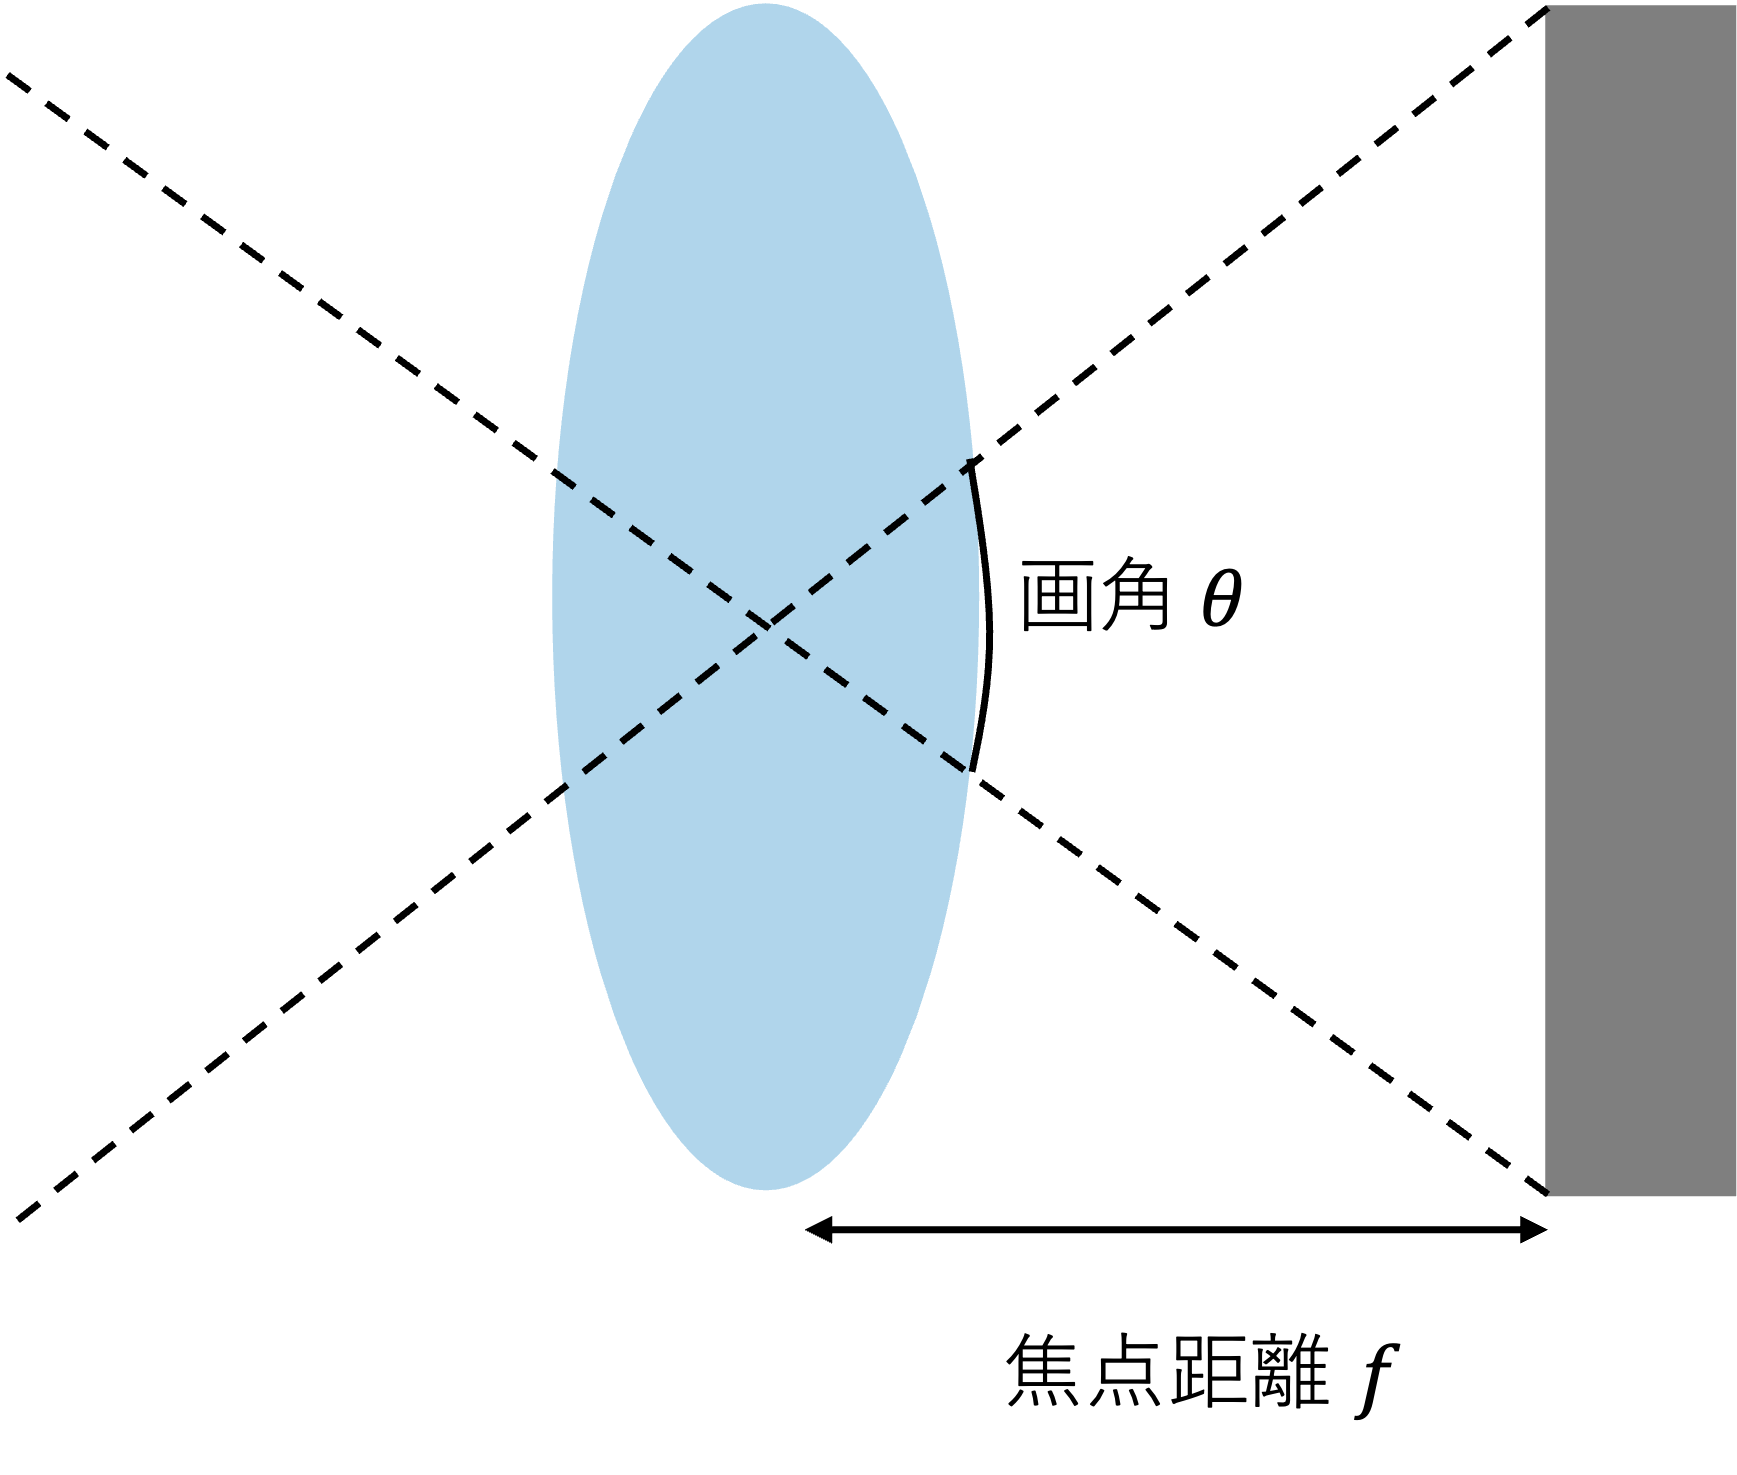
\includegraphics[width=0.4\textwidth]{figure/01.png}
      \caption{画角と焦点距離の関係}
      \label{fig:01}
  \end{figure}
\end{frame}

\begin{frame}{画角の求め方}
  \begin{block}{}
    画角は以下の公式を用いて求めることができる.
    \begin{equation}
      \theta = 2 \tan^{-1}{\dfrac{S / 2}{f}}
    \end{equation}
  \end{block}

  \begin{block}{}
    三角関数より,
    \begin{align*}
      \tan{\dfrac{\theta}{2}} &= \dfrac{S / 2}{f} \\
      \theta &= 2 \tan^{-1}{\dfrac{S / 2}{f}}
    \end{align*}
  \end{block}

  \begin{figure}[H]
    \centering
    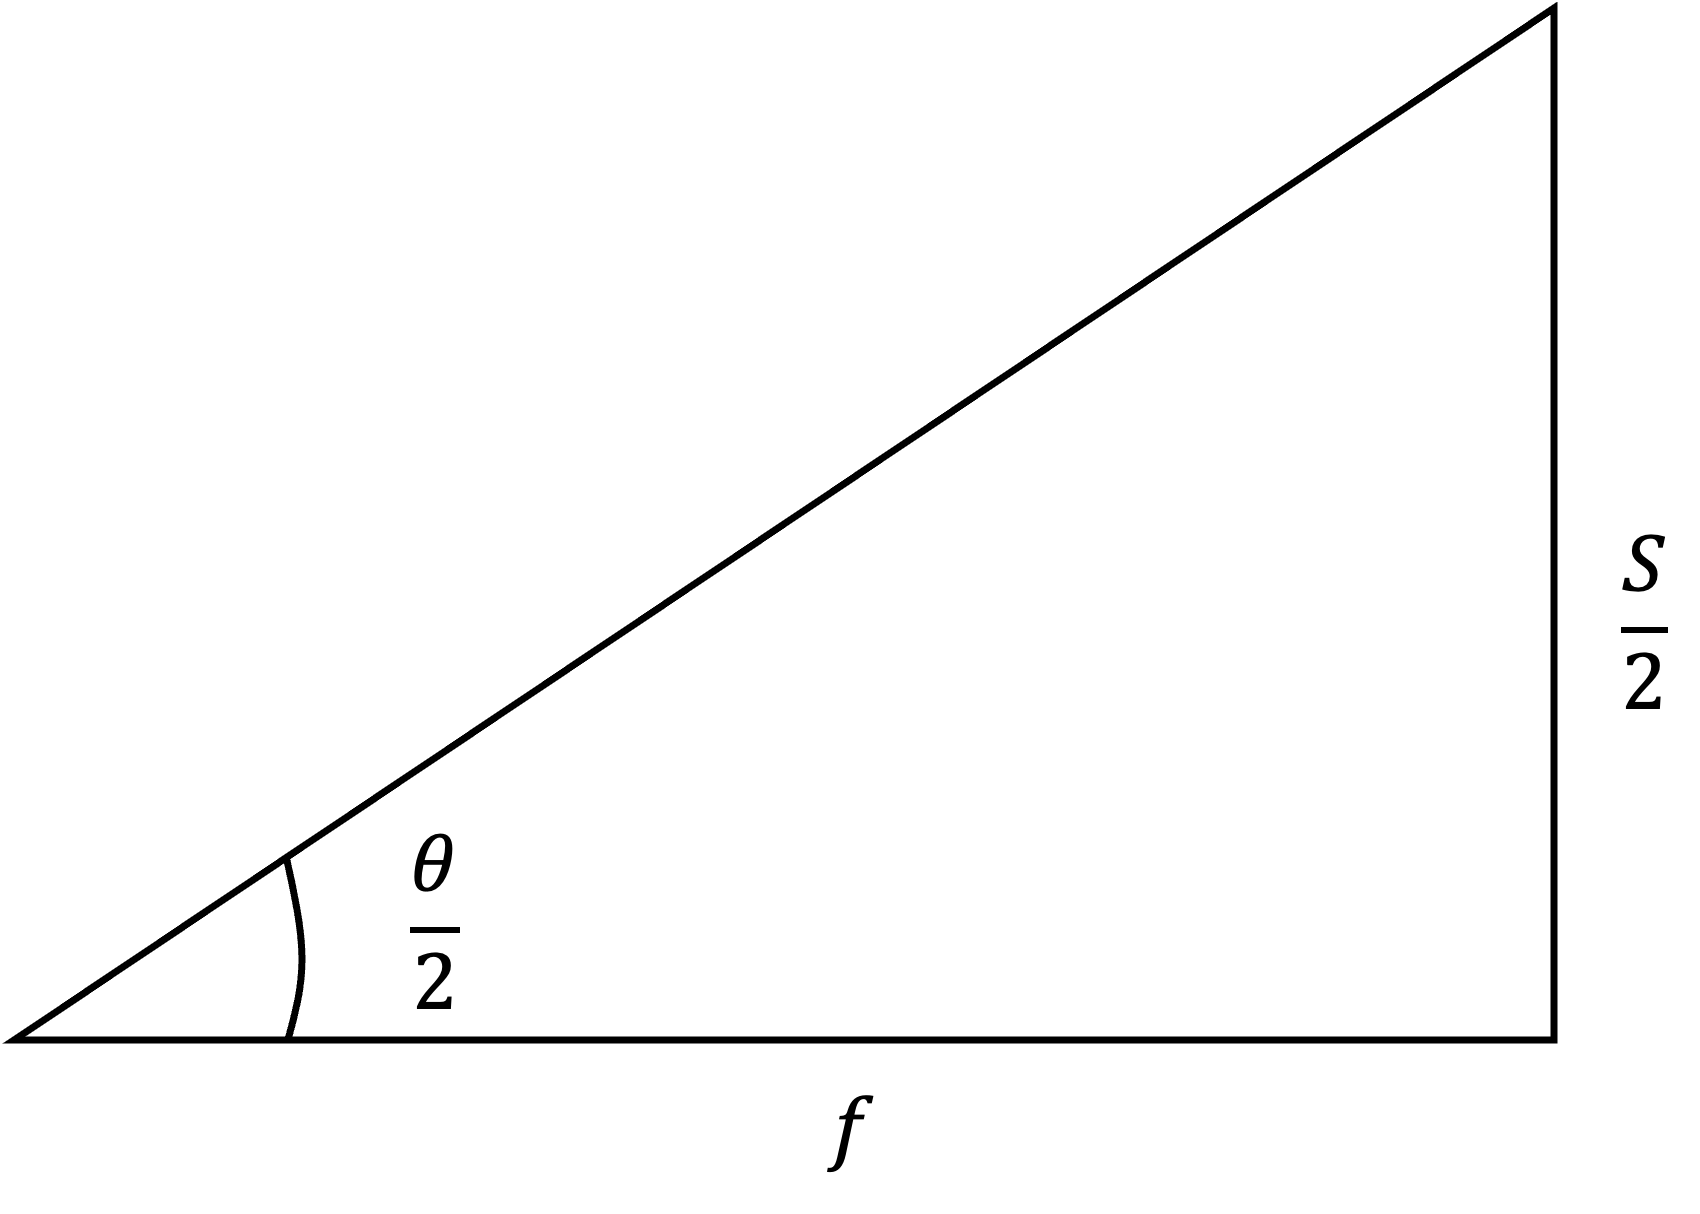
\includegraphics[scale=0.3]{figure/02.png}
    \caption{画角の求め方}
    \label{fig:02}
  \end{figure}
\end{frame}

\begin{frame}{撮像素子}
  \begin{block}{撮像素子とは}
    被写体の光を電気信号に変換する部品のことを示す.撮像素子サイズは変更や調整ができない為,カメラを選定することによって撮像素子サイズが決定する.主に,インチやフィルムサイズをもとに表される.
  \end{block}

  \begin{table}[H]
    \centering
    \caption{写真撮影酔うカメラで使用されている代表的な撮像素子サイズ}
    \begin{tabular}{|l|lll|}
      \hline
      撮像素子サイズ & 横 & 縦 & 対角線 \\
      \hline
      1/2.7インチ & 5.28mm & 3.96mm & 6.6mm \\
      1/1.8インチ & 7.2mm & 4.8mm & 8.7mm \\
      フォーサーズ & 17.3mm & 13.0mm & 21.6mm \\
      APS-C(キヤノン) & 22.3mm & 14.9mm & 26.8mm \\
      APS-C(ソニー、ニコン) & 23.6mm & 15.8mm & 28.4mm \\
      APS-H(キヤノン) & 28.1mm & 18.7mm & 33.8mm \\
      フルサイズ & 36.0mm & 24.0mm & 43.3mm \\
      \hline
    \end{tabular}
  \end{table}
\end{frame}


\begin{frame}{レンズ焦点距離}
  \begin{block}{レンズ焦点距離とは}
    レンズの後側主点から後側焦点までの距離のことを指す.
    レンズ焦点距離が長いほど,被写体は大きく撮影される.
    レンズ書店距離が短いほど,被写体は小さく撮影され,撮影できる範囲は広い.
  \end{block}

  \begin{figure}[H]
    \centering
    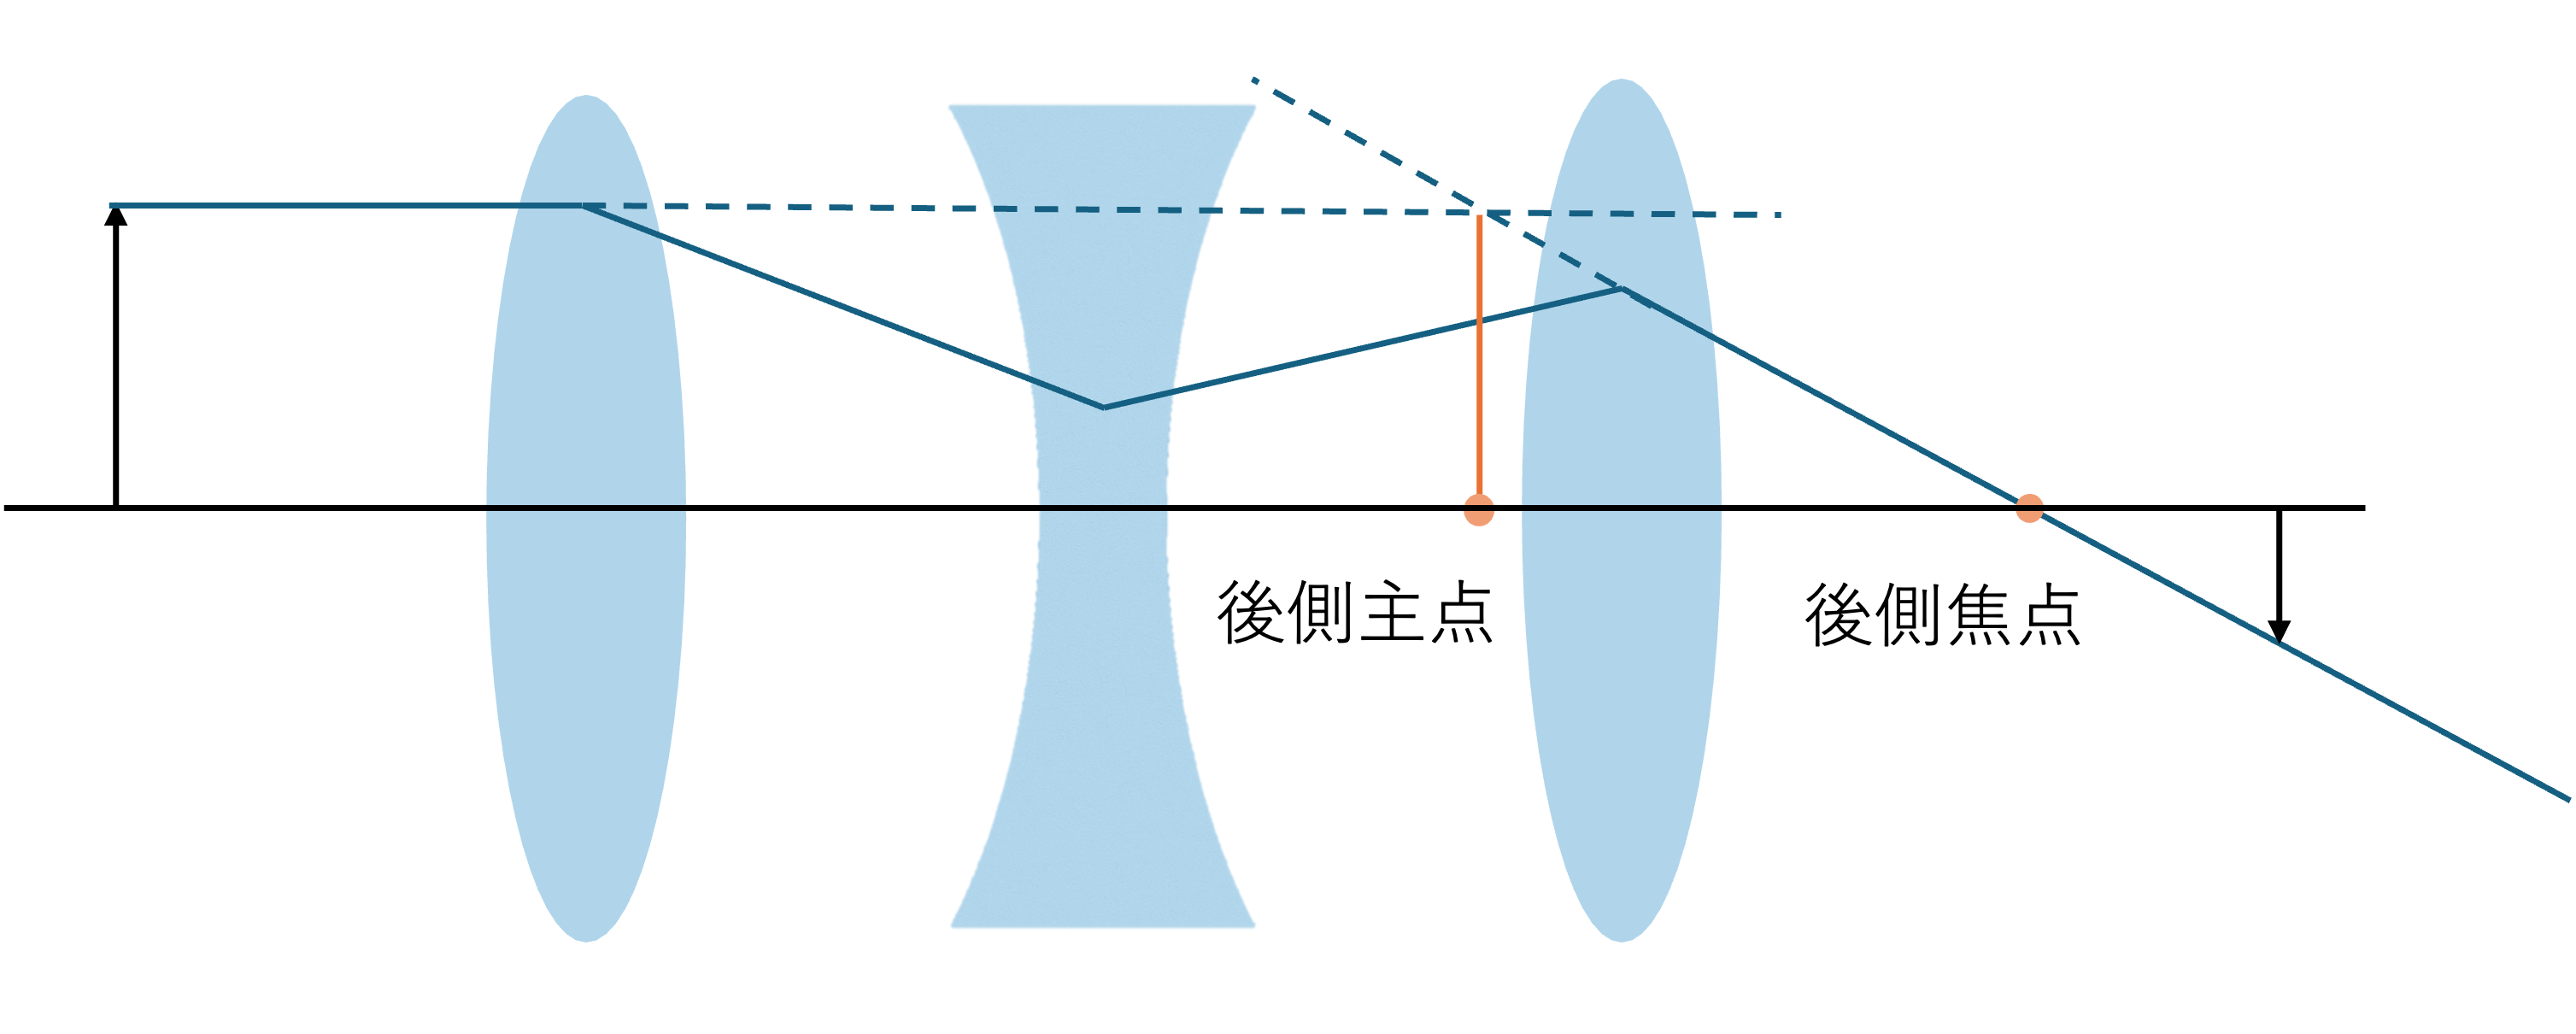
\includegraphics[scale=0.3]{figure/04.png}
    \caption{後側主点と後側焦点}
    \label{fig:04}
  \end{figure}
\end{frame}

\begin{frame}[allowframebreaks]{焦点距離の換算}
  \begin{block}{35mm換算焦点距離}
    同じ焦点距離のレンズを用いても撮像素子サイズに応じ,撮影画角が変化するため,レンズ焦点距離だけでは撮影画角は分からない.
    そこで,35mm換算焦点距離を用いることで,撮像素子サイズに対する撮影レンズの焦点距離を表す事ができる.
  \end{block}
  \newpage

\begin{block}{求め方}
  \tiny
  実際の焦点距離と35mm換算焦点距離は相似として考えることができるため,以下の式で求めることができる.
  \begin{align*}
    \dfrac{S / 2}{f} &\risingdotseq \dfrac{S_{35} / 2}{f_{35}} \\
    \dfrac{f}{S} &\risingdotseq \dfrac{f_{35}}{S_{35}}  \\
    f_{35} &\risingdotseq \dfrac{S_{35}}{S}f
  \end{align*}
  ここで, $S_{35} = \sqrt{36^2 + 24^2}$ であるため,代入すると
  \begin{align*}
    f_{35} \risingdotseq \dfrac{\sqrt{36^2 + 24^2}}{S} f = \dfrac{43.3}{S}f
  \end{align*}
\end{block}
\begin{figure}[H]
  \centering
  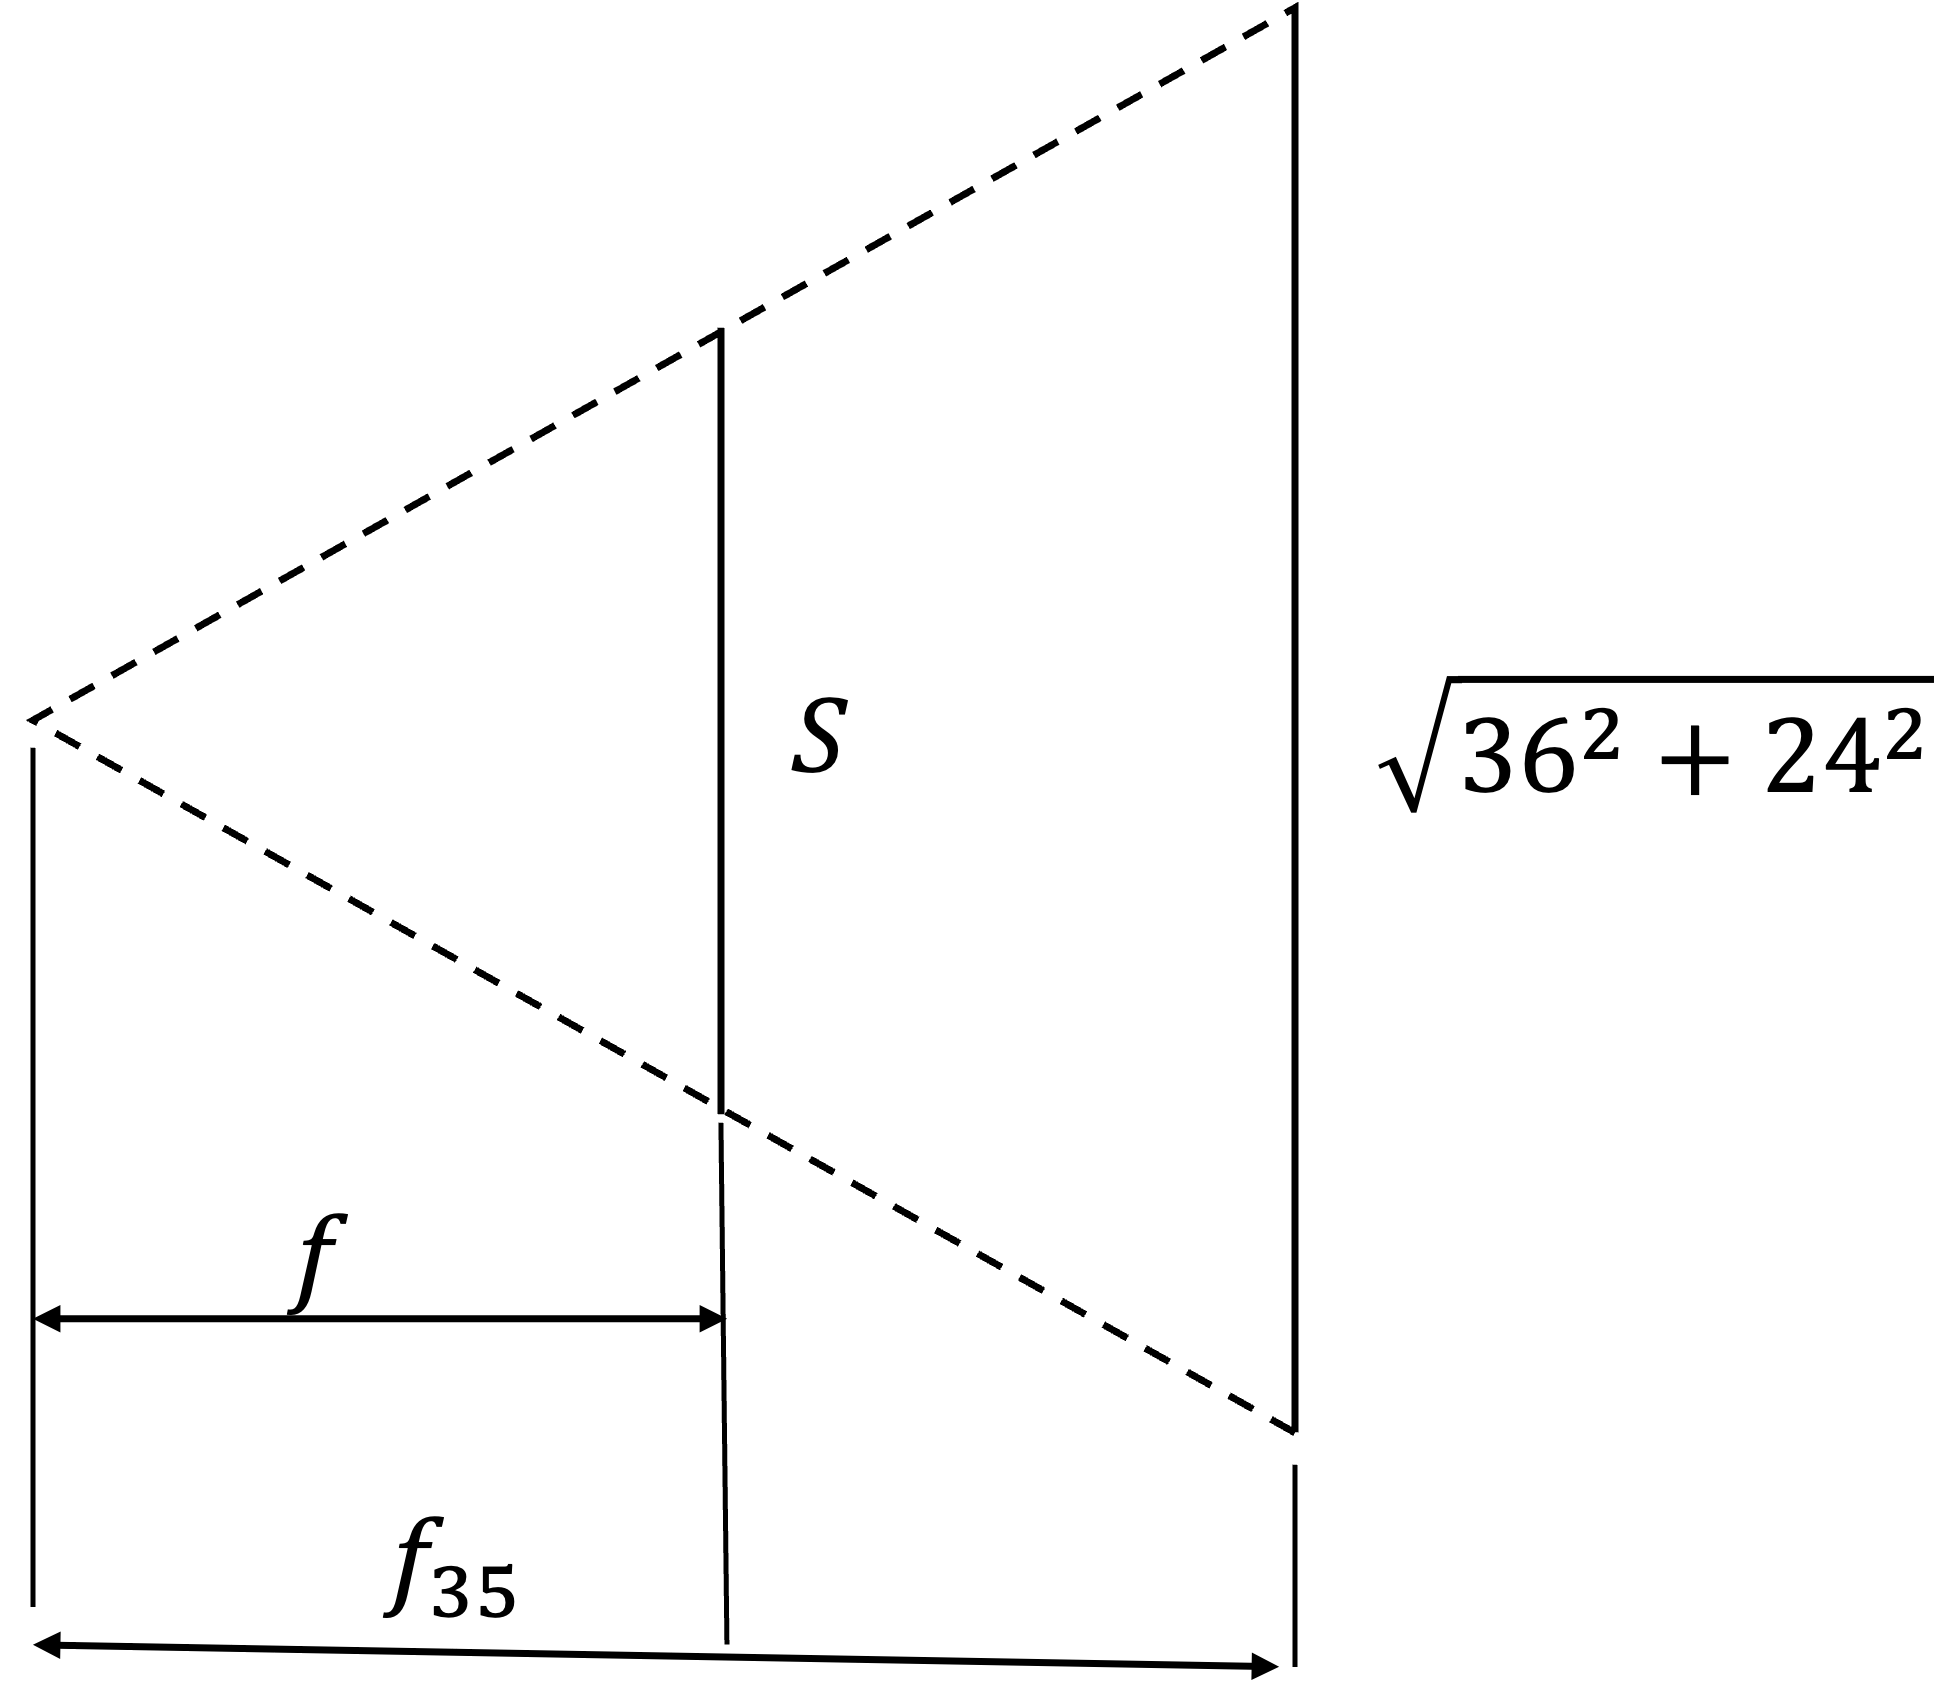
\includegraphics[scale=0.137]{figure/03.png}
  \caption{焦点距離 $f$ と 35mmフィルム換算焦点距離 $f_{35}$ の関係}
  \label{fig:03}
\end{figure}
\end{frame}

\begin{frame}{35mmフィルム換算焦点距離}
  35mmフィルム換算焦点距離では,以下のように分けて呼ばれることがある.
  \begin{table}[H]
    \centering
    \caption{35mmフィルム換算焦点距離での区分け}
    \begin{tabular}{|l|l|}
      \hline
      区分け & 35mmフィルム換算焦点距離 \\
      \hline
      広角レンズ & \textasciitilde ~ 50 \\
      標準レンズ & 50前後 \\
      望遠レンズ & 50 ~ \textasciitilde \\
      \hline
    \end{tabular}
  \end{table}
\end{frame}


\section{画像の明るさ}
\begin{frame}{画像の明るさ}
\begin{block}{}
  撮影レンズで集光して撮像素子上に像が結像する際,撮影レンズの直径とレンズ焦点距離によって像の明るさは異なる.像の明るさは,撮影レンズの直径 $D$ の2乗に比例している.また,撮像レンズの焦点距離 $f$ の2乗に反比例している.
  \begin{equation}\label{ip}
    I \propto (\dfrac{D}{f})^2
  \end{equation}
\end{block}
\end{frame}

\begin{frame}{Fナンバ}
  \begin{block}{}
    Fナンバとは,撮影レンズの焦点距離 $f$ をレンズの直径 $D$ で割った値であり,撮影レンズの集光性能を表す.
    また,レンズ絞りで設定したFナンバをレンズの絞り値と呼ぶ.
    \begin{equation} \label{fnam}
      F\text{ナンバ} = \dfrac{f}{D}
    \end{equation}
  \end{block}

  \begin{block}{画像の明るさとFナンバの関係}
    \eqref{ip}と\eqref{fnam}より,\eqref{if}の式を導くことができる.
    \begin{equation} \label{if}
      I \propto \dfrac{1}{F\text{ナンバ}^2}
    \end{equation}
  \end{block}
\end{frame}

\begin{frame}{シャッタースピード}
  \begin{block}{}
    シャッタスピードとは,画像を撮影するために撮像面上に光を当てる時間の事を指す.撮像素子が受け取る光エネルギーは,光量 $\times$ 時間 と考えることができるので,
    シャッタスピードを1段階遅くすると,光が当たる時間が2倍になるため,画像の明るさも2倍になる.
  \end{block}
  \begin{table}[h]
    \centering
    \caption{シャッタスピード}
    \begin{tabular}{|c|c|c|c|c|c|c|c|c|c|}
      \hline
      1/1,000 & 1/500 & 1/250 & 1/125 & 1/60 & 1/30 & 1/15 & 1/8 & 1/4 & 1/2 \\
      \hline
    \end{tabular}
  \end{table}
\end{frame}

\begin{frame}{ISO感度}
  \begin{block}{}
    光に対するフィルム感度を表したもの.フィルム感度は100を基準として100に対して2倍の感度があれ200となる.産業用カメラの場合はISO感度の代わりにゲイン\footnote{増幅器の倍率を示す}を用いる.
    撮像素子から読みだした信号には画像情報と共にノイズが含まれており,ISO感度を2倍にすると信号が増幅されるがノイズも増加する.したがって,感度をあげると共に画像中のノイズも多くなる.
  \end{block}
  \begin{figure}[htbp]
      \centering
      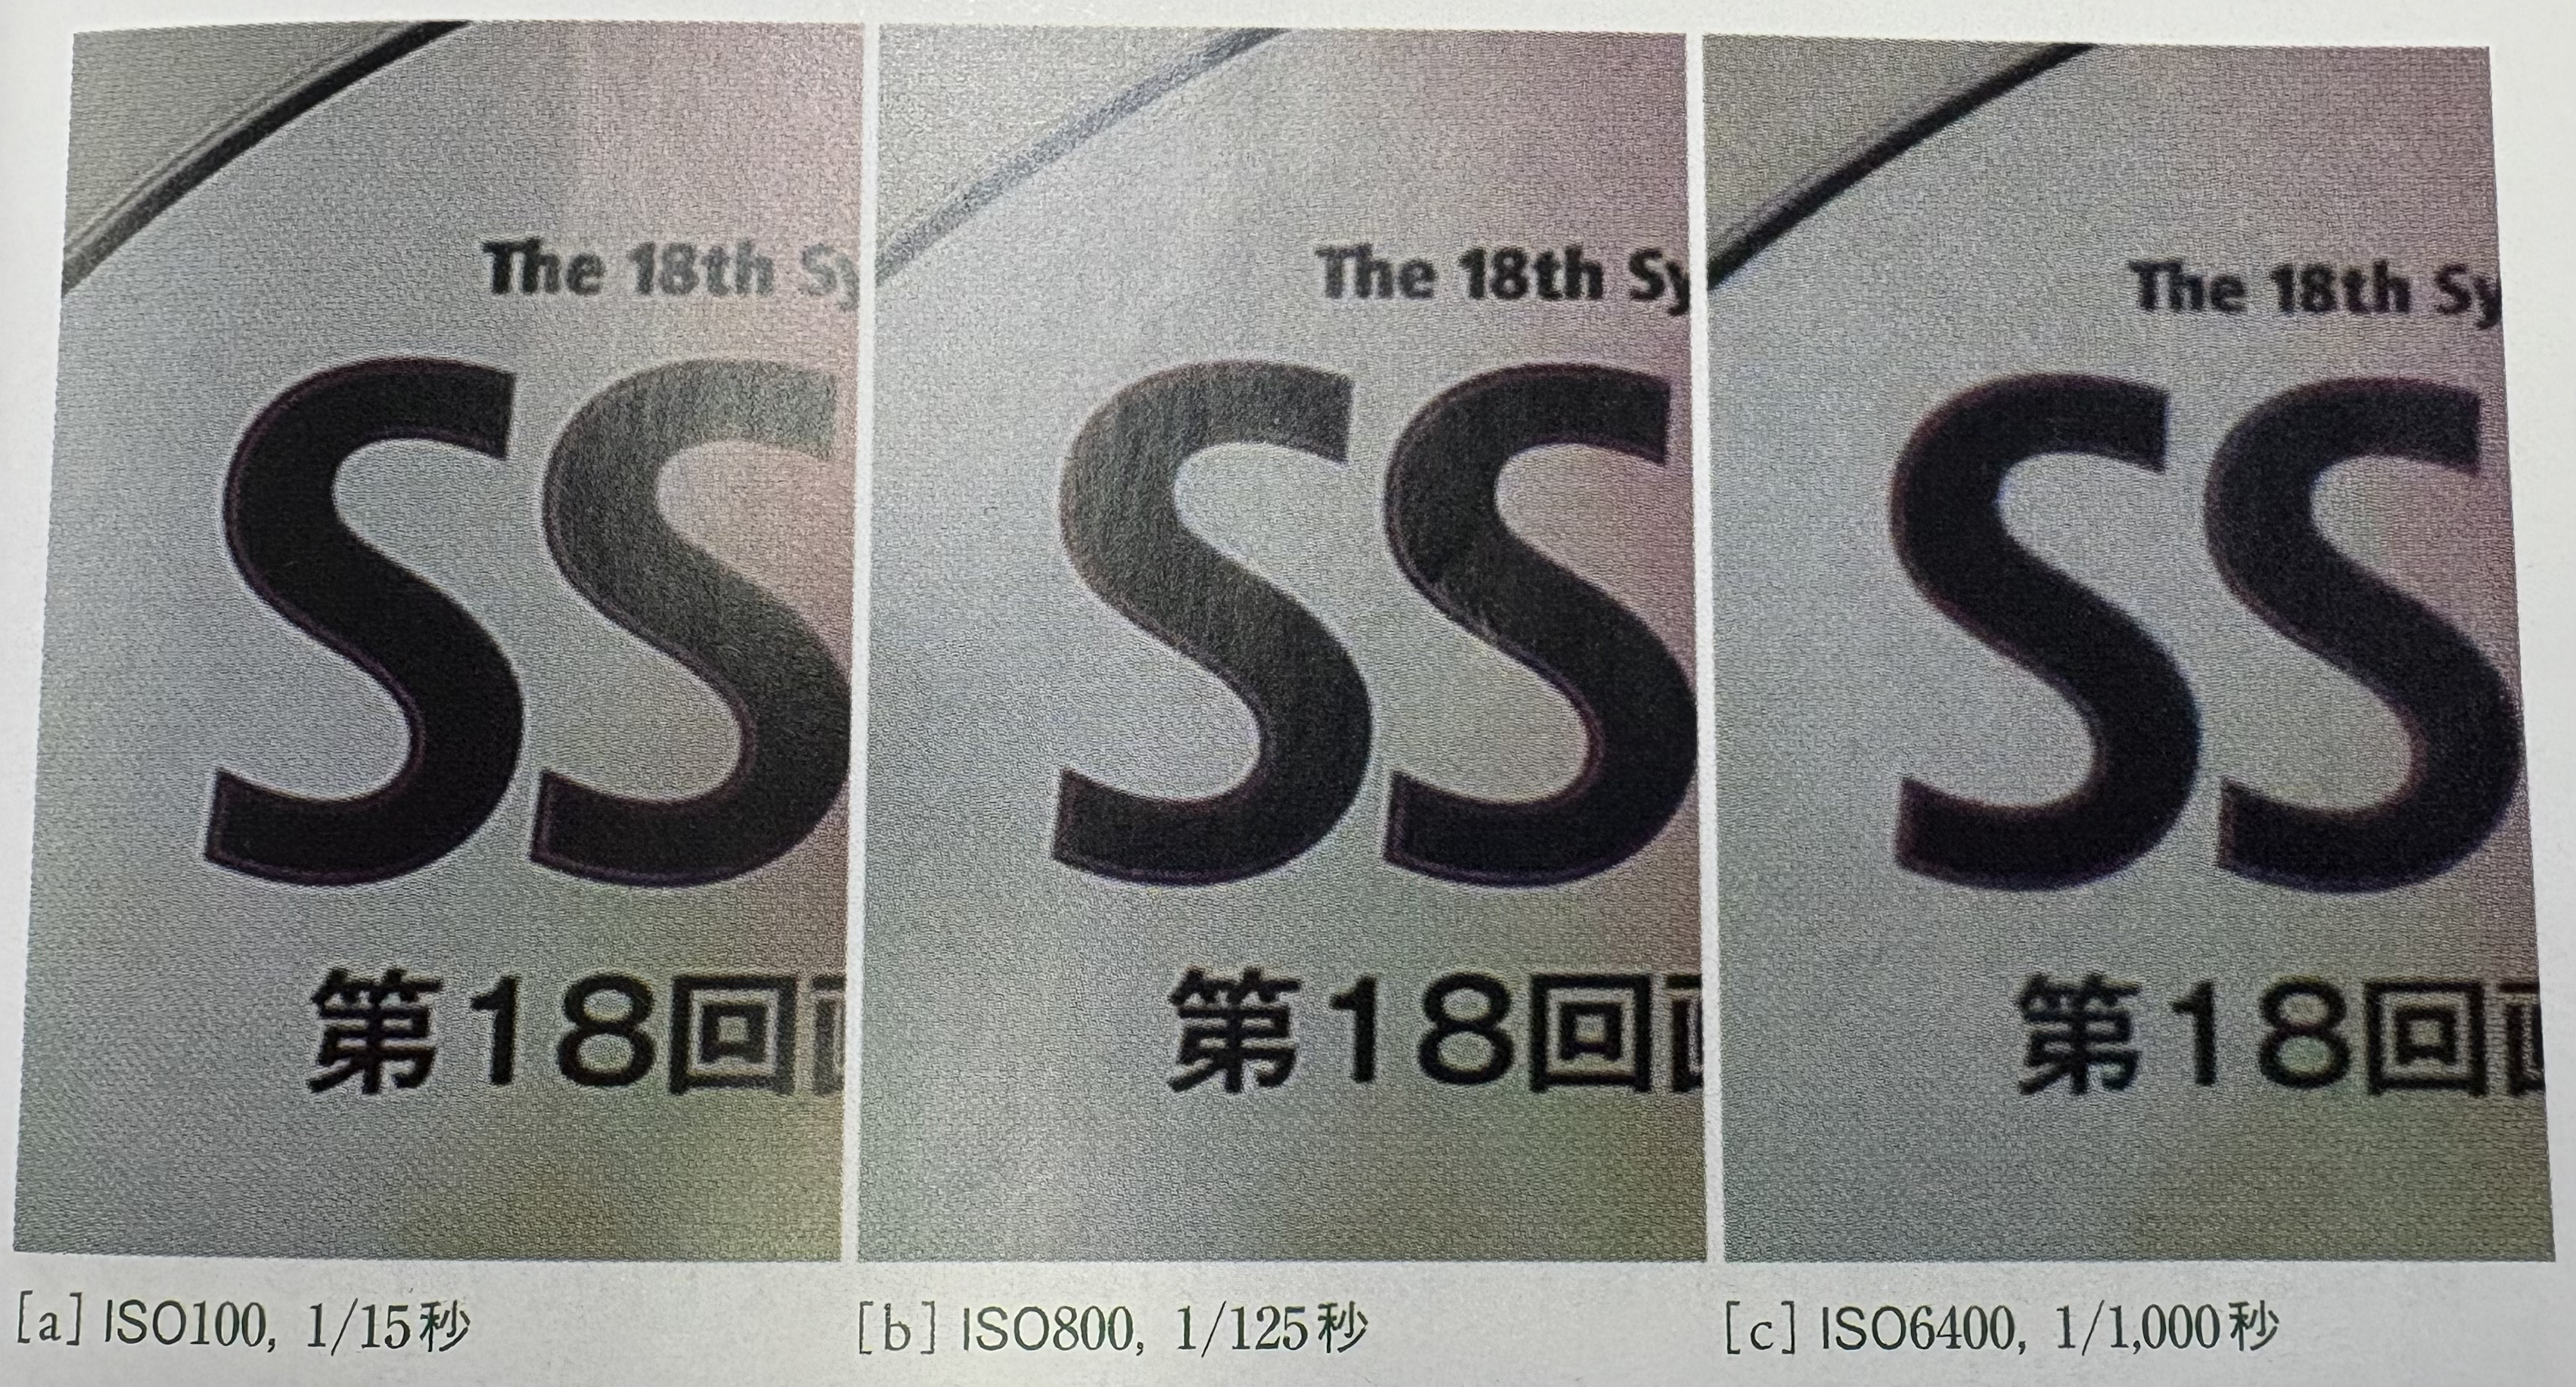
\includegraphics[keepaspectratio,width=0.5\textwidth]{figure/013.jpg}
      \caption{ISO感度の違いによるノイズの変化}
      \label{fig:label}
  \end{figure}
\end{frame}

\begin{frame}[allowframebreaks]{移動ブレの防止}
  画像の明るさを同じするためには以下のような要素を組み合わせて使用することができる.したがって,画像を撮影する際には,目的に応じた設定が必要である.
  この目的の1つとしてブレのない画像を撮影することである.被写体が移動する移動ブレは,シャッタスピードをより短時間に設定することで防ぐことが可能である.
  \begin{itemize}
    \item 絞り値
    \item シャッタスピード
    \item ISO感度
    \item 焦点距離
    \item 撮影レンズの直径
  \end{itemize}

  \newpage
  \begin{exampleblock}{被写体の移動ブレがない画像の取り方}
    \tiny
    以下のように変数を定義した際の移動ブレが十分に小さいシャッタスピードは\eqref{ts}で求めることができる.
    \begin{itemize}
      \item 被写体までの距離 $R[m]$
      \item 被写体の移動速度 $v[m]$
      \item シャッタスピード $t_s[s]$
      \item レンズ焦点距離 $f[mm]$
      \item 撮像素子サイズ $S[mm]$
      \item 撮像素子サイズに対応する方向の画素数 $N$
    \end{itemize}
    \begin{equation}\label{ts}
      \begin{split}
        vt_s : R &= \dfrac{S}{N} : f \\
        t_s &= \dfrac{S}{N} \cdot \dfrac{R}{vf}
      \end{split}
    \end{equation}
  \end{exampleblock}

  \begin{figure}[H]
    \centering
    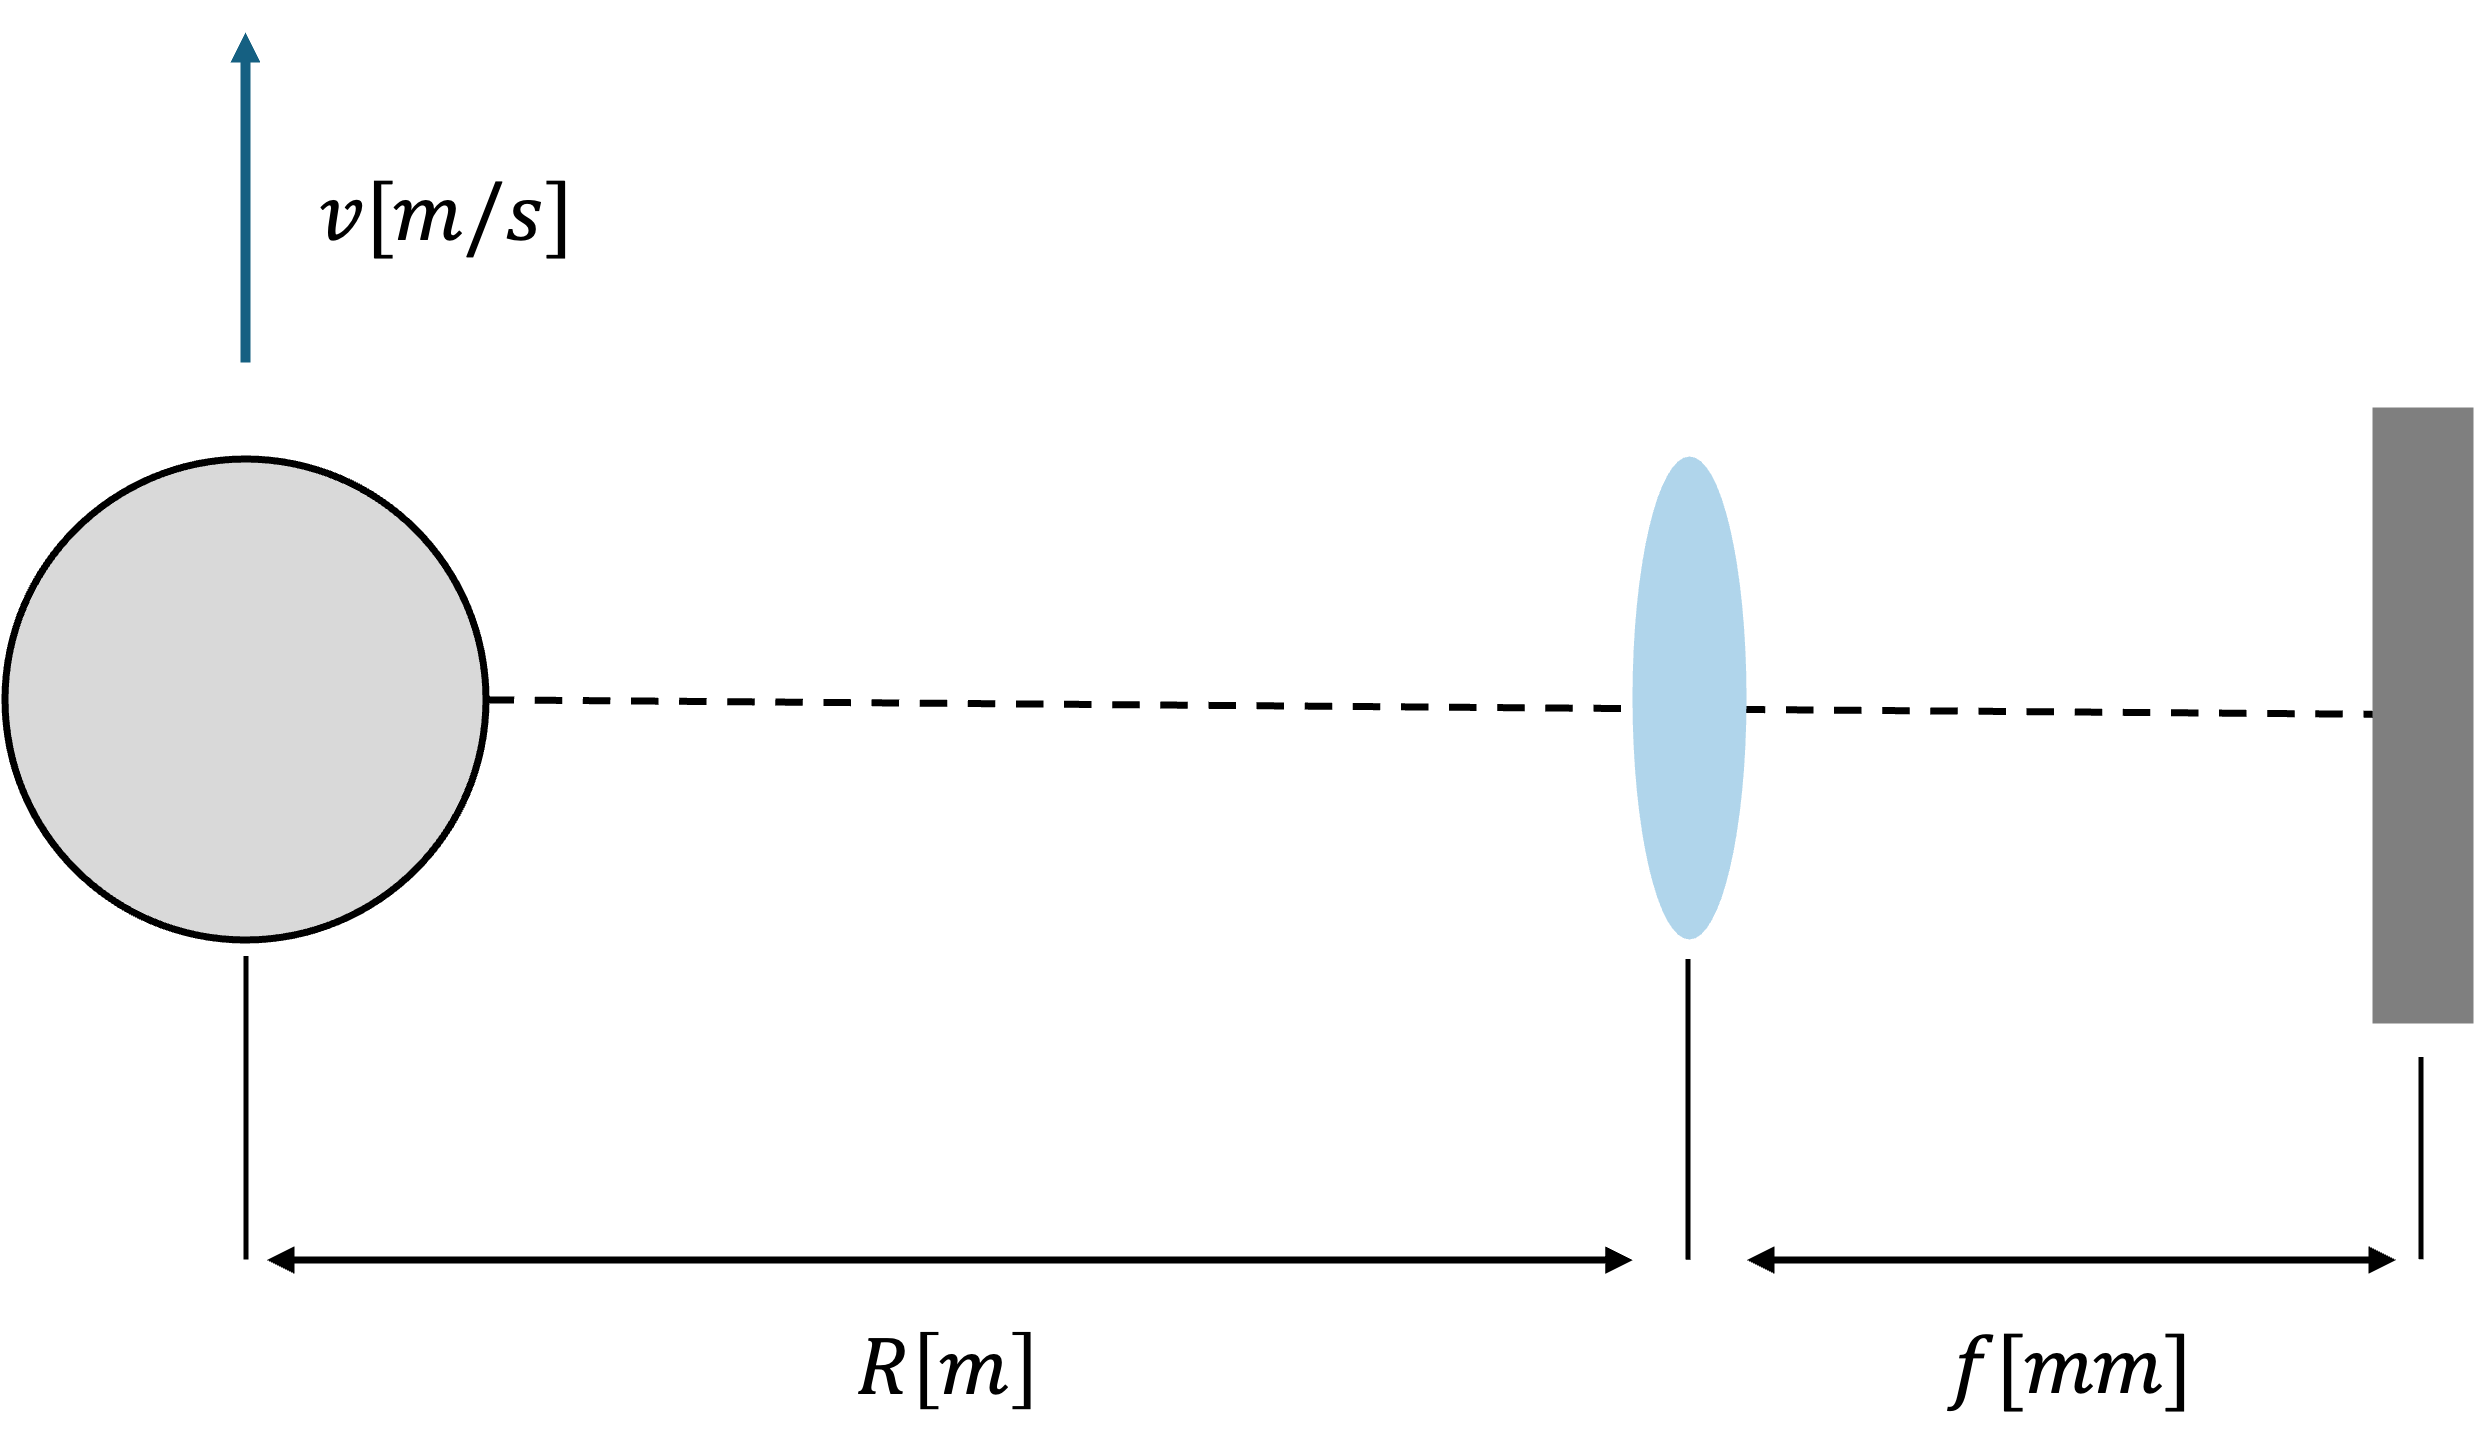
\includegraphics[scale=0.21]{figure/05.png}
    \caption{移動する被写体をぶれなく撮影できるシャッタスピードを求める}
    \label{fig:05}
  \end{figure}

  \newpage

  \begin{exampleblock}{変数の入力例}
    先ほどの変数をそれぞれ以下のような場合のときに考えてみる.
    \begin{itemize}
      \item $R = 10[m]$
      \item $ v = 10[m/s]$
      \item $f = 6[mm]$
      \item $S = 4.8[mm]$
      \item $N = 640$ $[$画素$]$
    \end{itemize}
    これらの値を\eqref{ts}に代入すると
    \begin{align*}
      10 \cdot t_s : 10 &= \dfrac{4.8}{640} : 6 \\
      t_s &= \dfrac{4.8}{640} \cdot \dfrac{10}{10 \cdot 6} \\
      t_s &= \dfrac{1}{800}
    \end{align*}
  \end{exampleblock}
\end{frame}

\section{被写界深度}

\begin{frame}[allowframebreaks]{被写界深度}
  \begin{block}{}
    被写界深度とは,写真においてピントが合って見える範囲のことを指す.カメラで撮影する際に完全にピントが合う面は理論上1点であるが,
    その前後にもピントが合って見える範囲がある.このピントが合って見える奥行きの範囲が被写界深度である.
  \end{block}

  図\ref{fig:a},図\ref{fig:b},図\ref{fig:c}では,レンズ主点 $O$ から距離 $a$ の位置の被写体 $A$ に対して,レンズ主点からレンズ焦点距離 $f$ よりも少し大きな位置 $b$ の位置にある
  撮像素子上にピントが合っている.


  \begin{figure}[H]
    \centering
    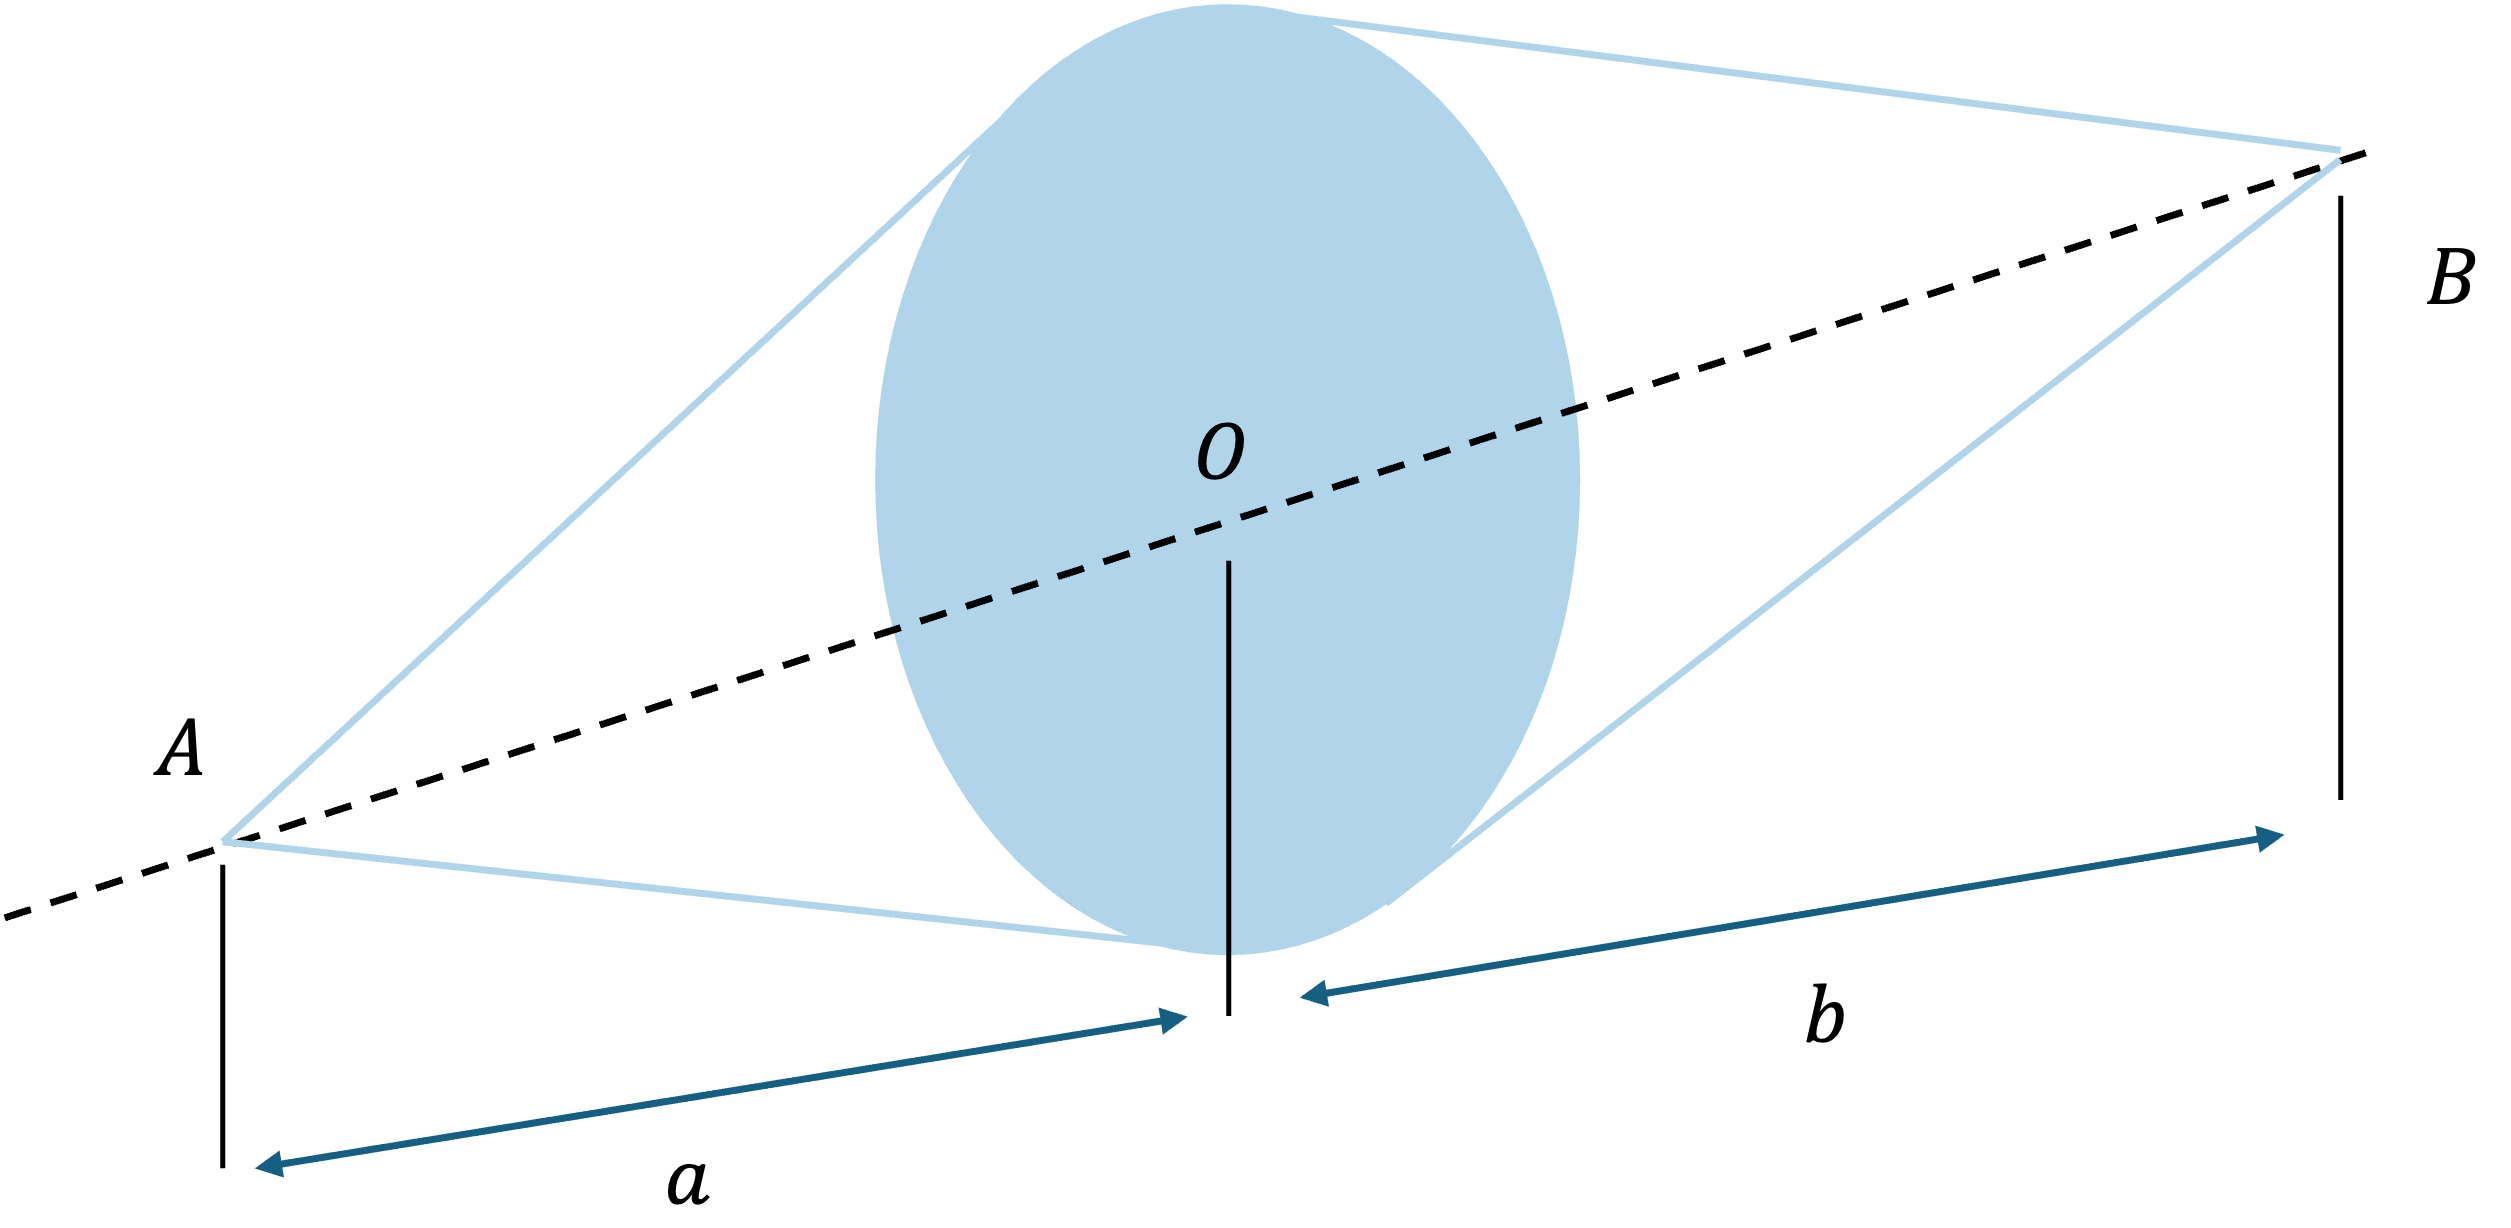
\includegraphics[scale=0.4]{figure/06.png}
    \caption{Aの位置の被写体は,撮像素子上にピントが合う}
    \label{fig:a}
  \end{figure}

  \newpage
  \begin{block}{図\ref{fig:b}について}
    次に,図\ref{fig:b}について考える.この場合では,被写体 $A$ よりも少し近い距離 $a_n$ にある被写体 $A_n$ について考える.
    被写体の位置が近づくと像の位置は焦点より後方で形成される.そのため,像ができるのは撮像素子よりも離れた距離 $b_n$ である.
\end{block}
  \begin{figure}[H]
    \centering
    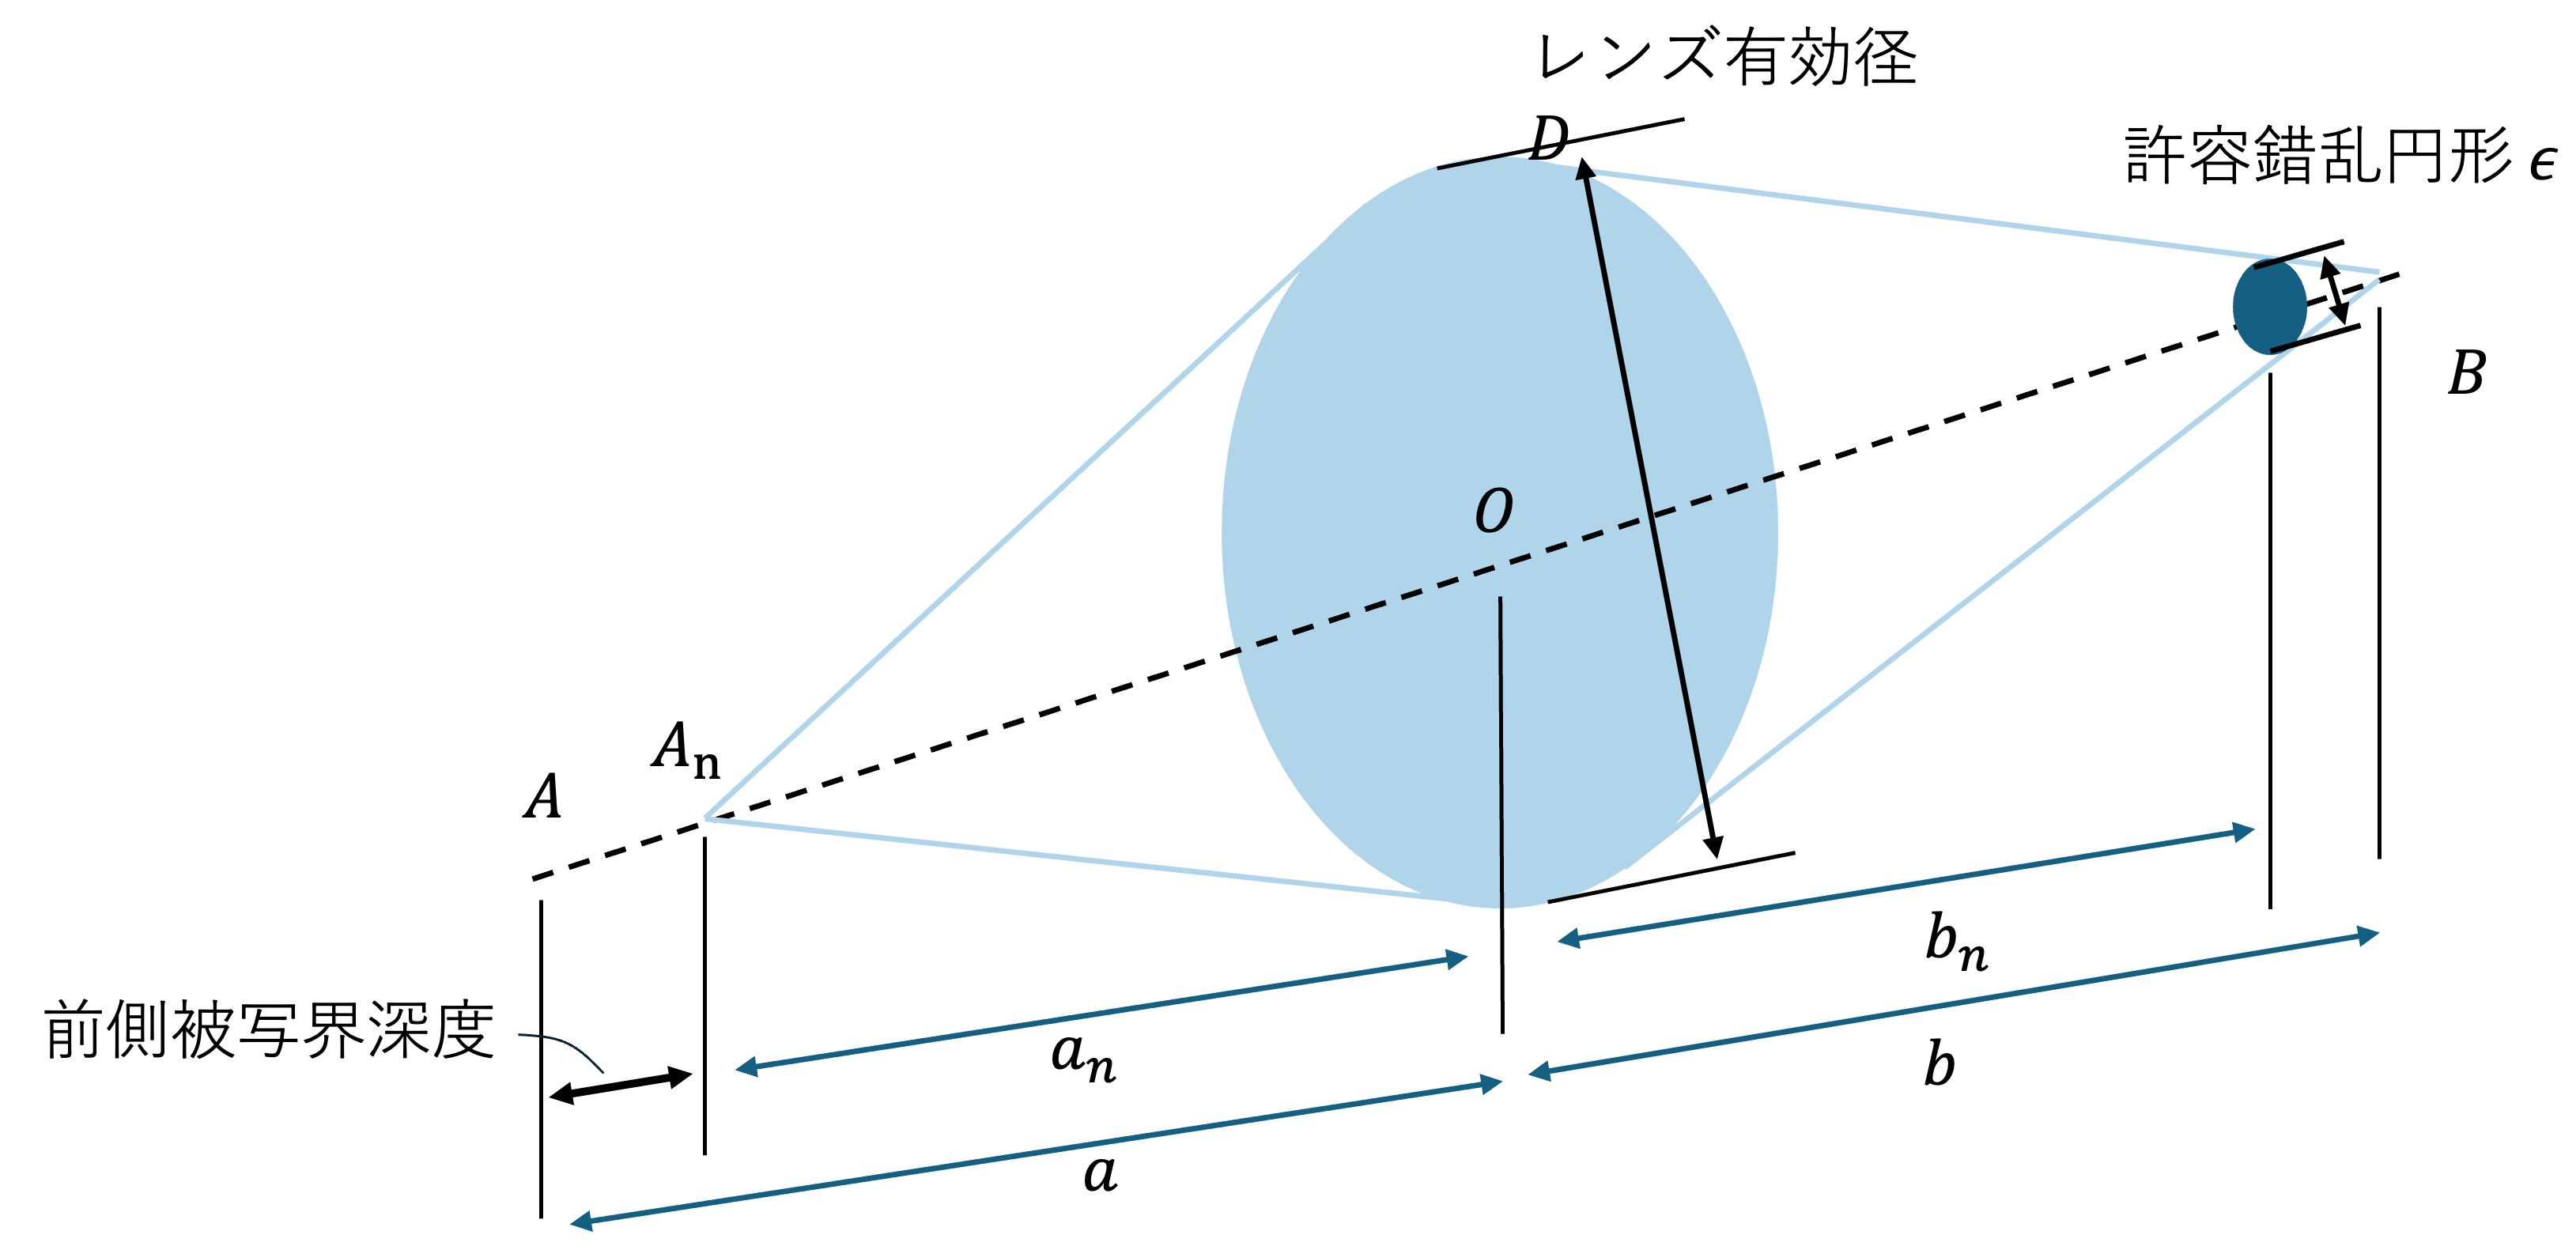
\includegraphics[scale=0.35]{figure/07.png}
    \caption{Aよりも近い位置の被写体は,撮像素子よりも後でピントが合う}
    \label{fig:b}
  \end{figure}
\newpage
  \begin{block}{図\ref{fig:c}について}
    最後に,図\ref{fig:c} について考える.この場合では,被写体 $A$ よりも少し遠い距離 $a_f$ にある被写体 $A_f$ について考える.
    被写体の位置が遠ざかると像の位置は焦点より前方で形成される.そのため,像ができるのは撮像素子よりレンズに近い $b_f$ である.
  \end{block}
  \begin{figure}[H]
    \centering
    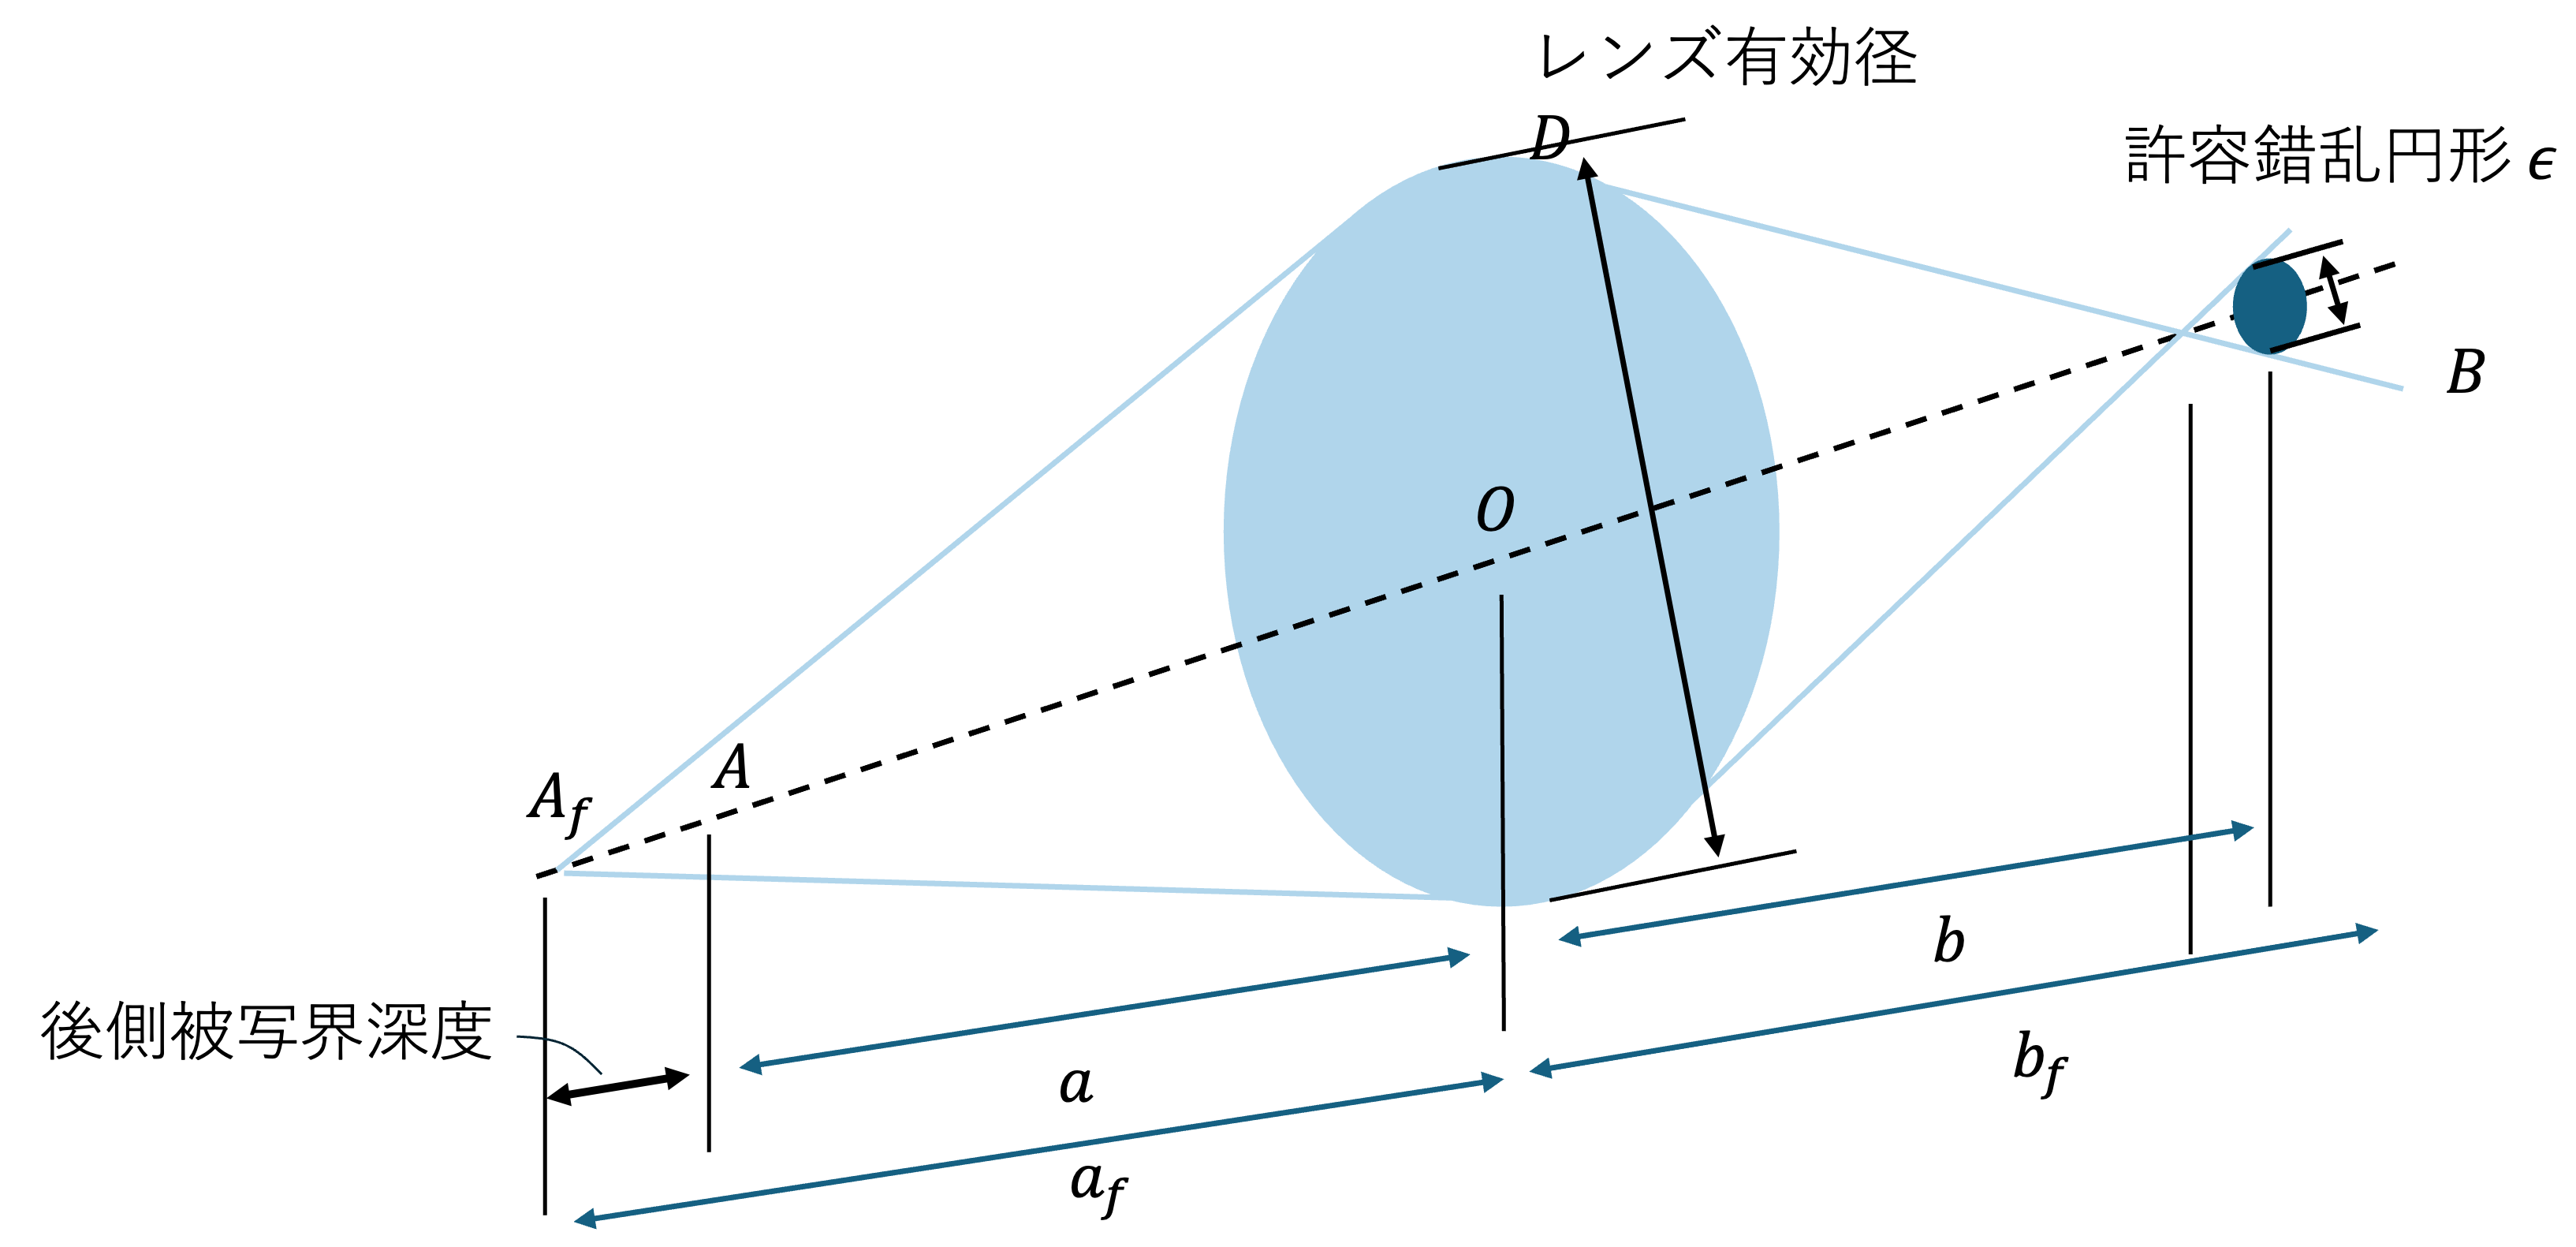
\includegraphics[scale=0.35]{figure/08.png}
    \caption{Aよりも遠い位置の被写体は,撮像素子よりも手前でピントが合う}
    \label{fig:c}
  \end{figure}

    \newpage

    \begin{block}{被写界深度の特性}
      被写界深度には以下のような特性がある.
      \begin{enumerate}
        \item 前側被写界深度よりも,後側被写界深度の方が深い
        \item 絞り値が同じなら,レンズ焦点距離が短いほど深く,長いほど浅い
        \item レンズ焦点距離が同じなら,絞り値が大きいほど深く,長いほど浅い
        \item 被写体距離が遠いほど深く,近いほど浅い.
      \end{enumerate}
    \end{block}

    \newpage
    \begin{block}{被写界深度についてのまとめ}
      被写界深度とは,遠点 $A_f$ から近点 $A_n$ までの実用上ピントが合っていると判断できる距離範囲の事である.
      また,$A$ から $A_f$ までを後側被写界深度,$A$ から $A_n$ までを前側被写界深度と言い,それらの和が被写界深度となる.
    \end{block}
    \begin{figure}[H]
      \centering
      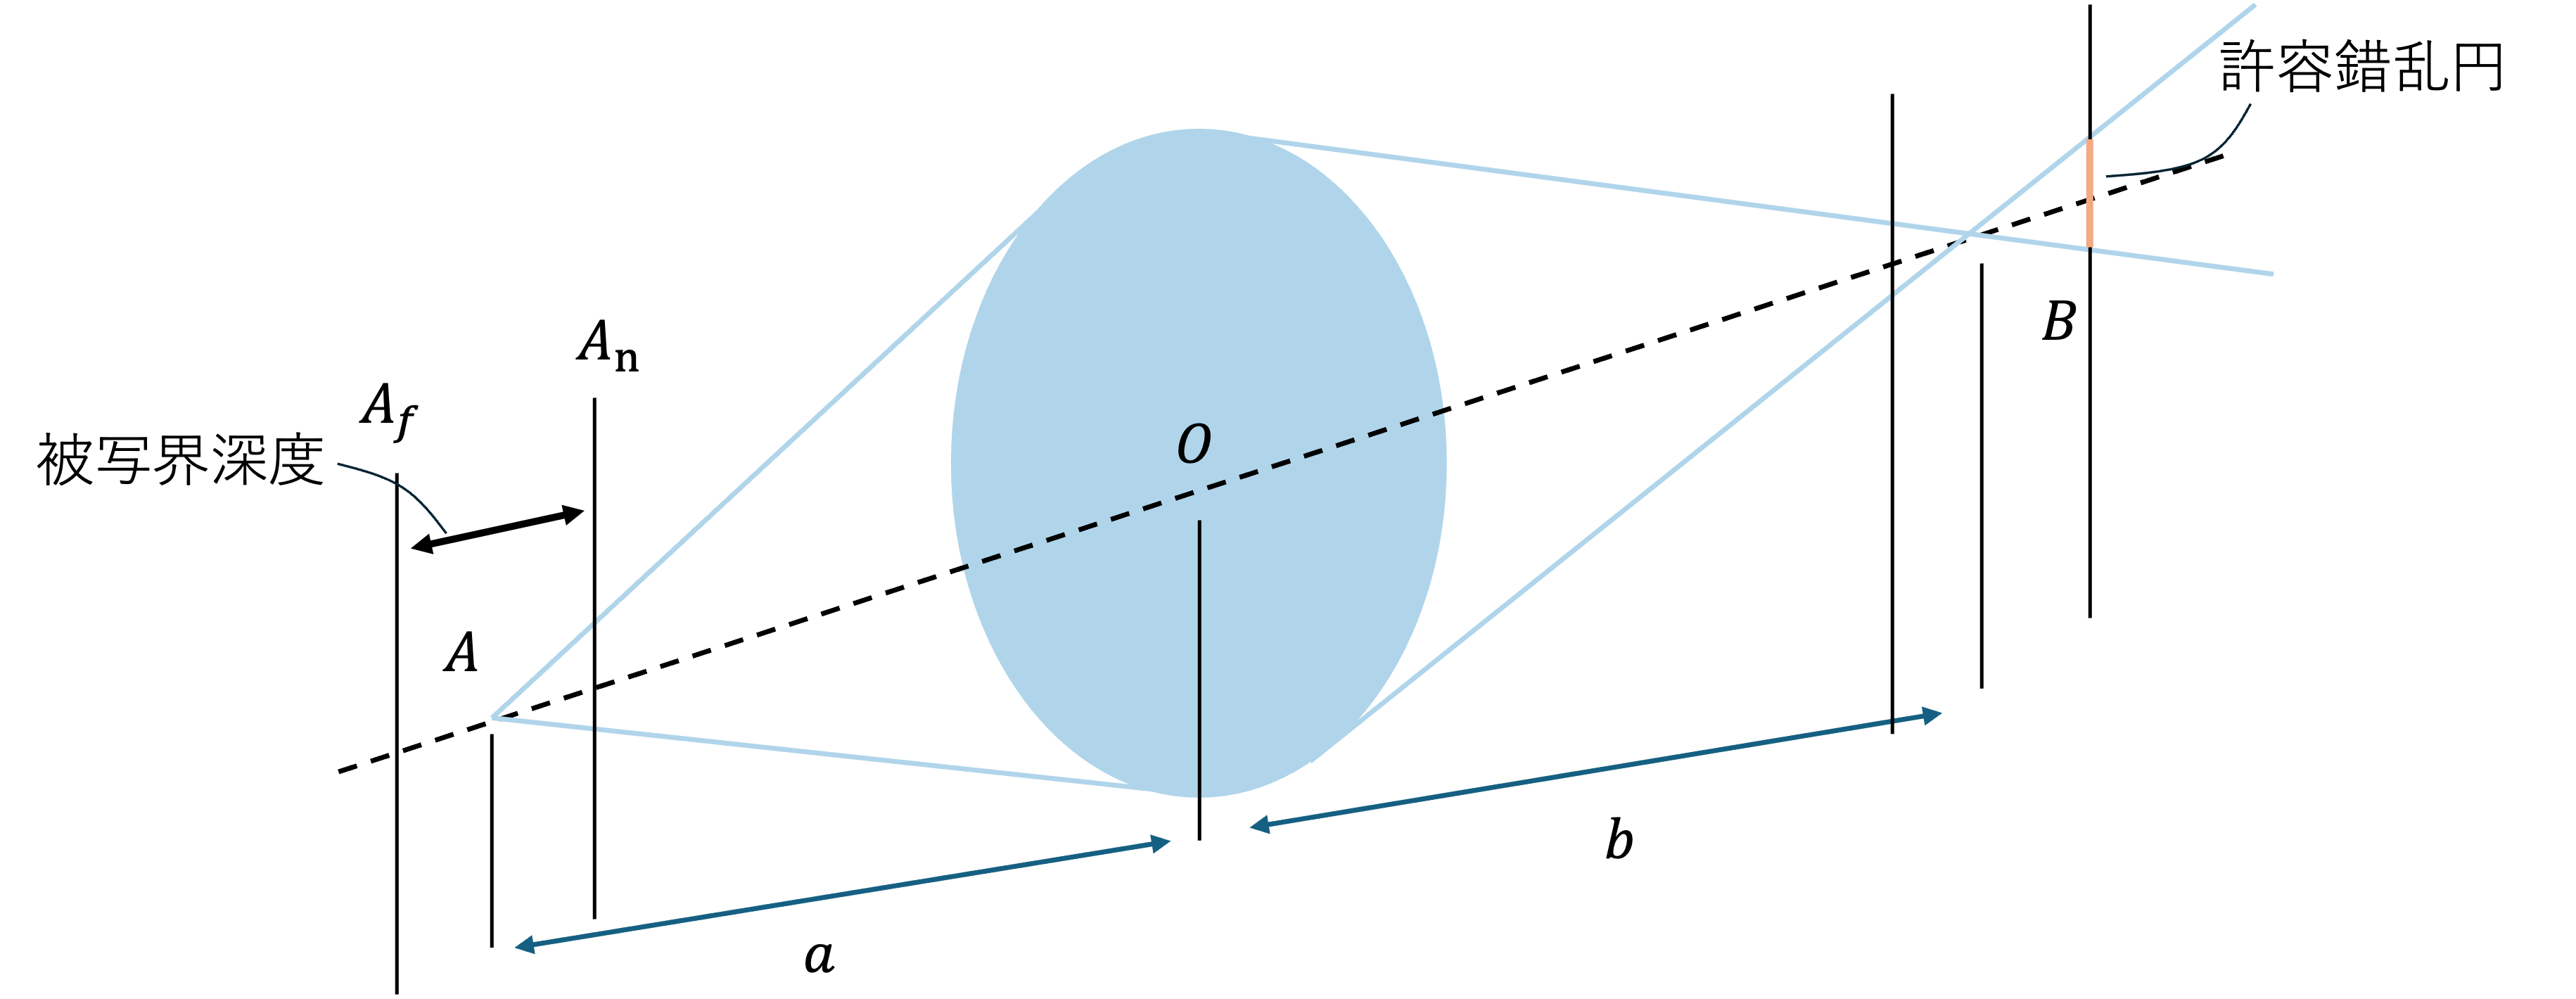
\includegraphics[scale=0.35]{figure/09.png}
      \caption{被写界深度のまとめ}
      \label{fig:09}
    \end{figure}

\end{frame}




\section{フレームレート}
\begin{frame}{フレームレート}
\begin{block}{}
  フレームレートとは,1秒あたりに切り替えて表示する画像枚数のことをフレームレートと呼び,単位にはfpsを用いる.
\end{block}
\begin{block}{フレームレートとシャッタースピードの関係性}
  電子シャッタを利用すると,連続した画像を撮影することができる.しかし,ある瞬間の露光が、次のフレームの露光時間と一部重なってしまうフレームの重複が発生してしまうため,電子シャッタのシャッタスピードはフレームレートに対する周期よりも長くすることができない.
\end{block}

\begin{figure}[H]
  \centering
  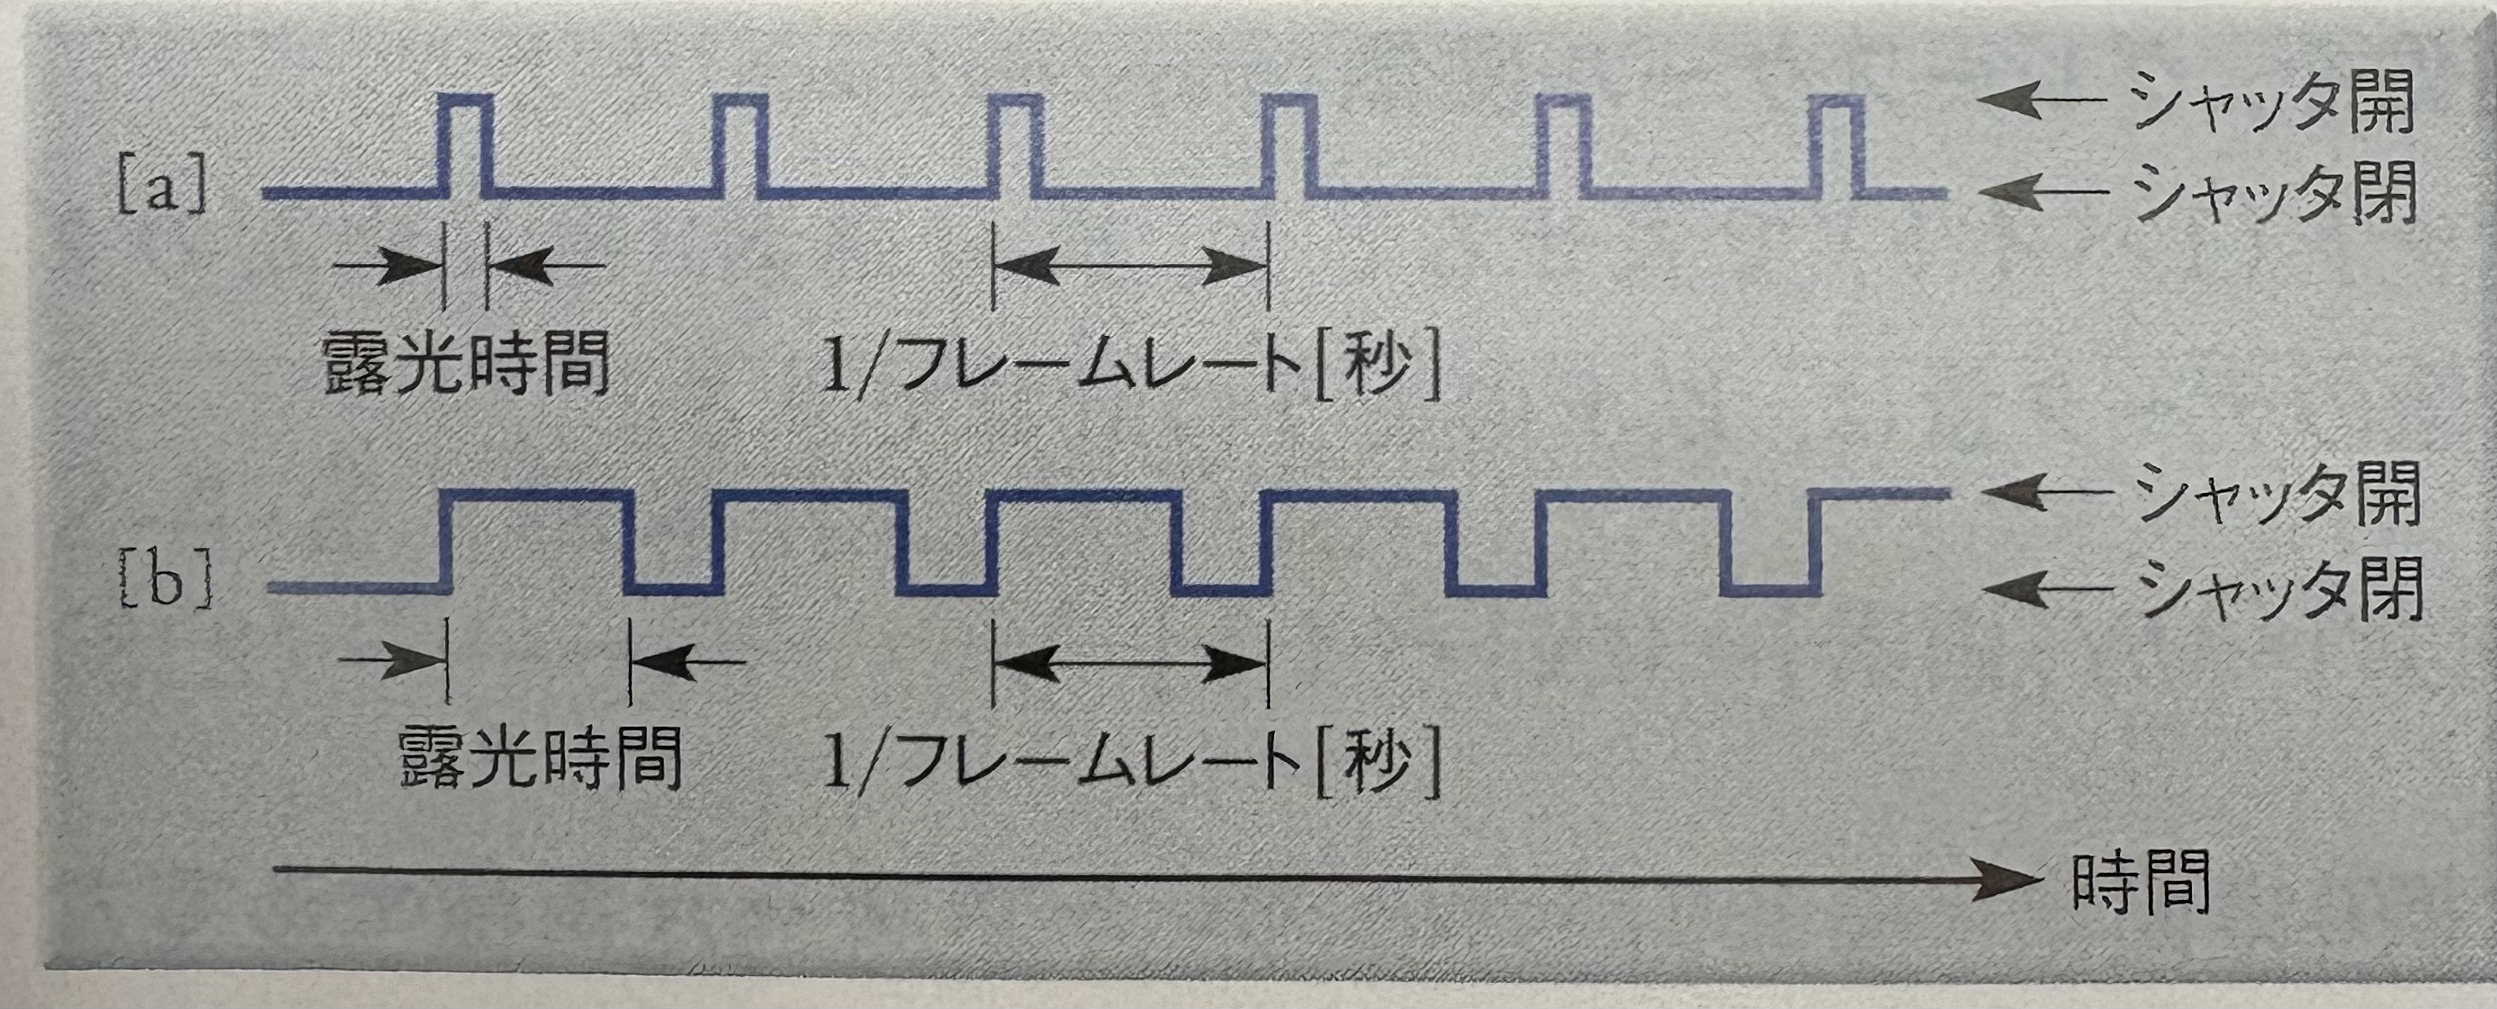
\includegraphics[width=0.5 \textwidth]{figure/011.jpg}
  \caption{露光時間とフレームレートの関係}
\end{figure}
\end{frame}

\begin{frame}{フリッカ}
  \begin{block}{}
    フリッカとは,照明が人の目には見えない早さで点滅している合間をカメラで撮影することで発生する画像のちらつき現象のこと.
    フリッカの現象は以下の例がある.
    \begin{itemize}
      \item 色が変化して写る
      \item 縞模様の発生
    \end{itemize}
  \end{block}
  \begin{figure}[H]
      \centering
      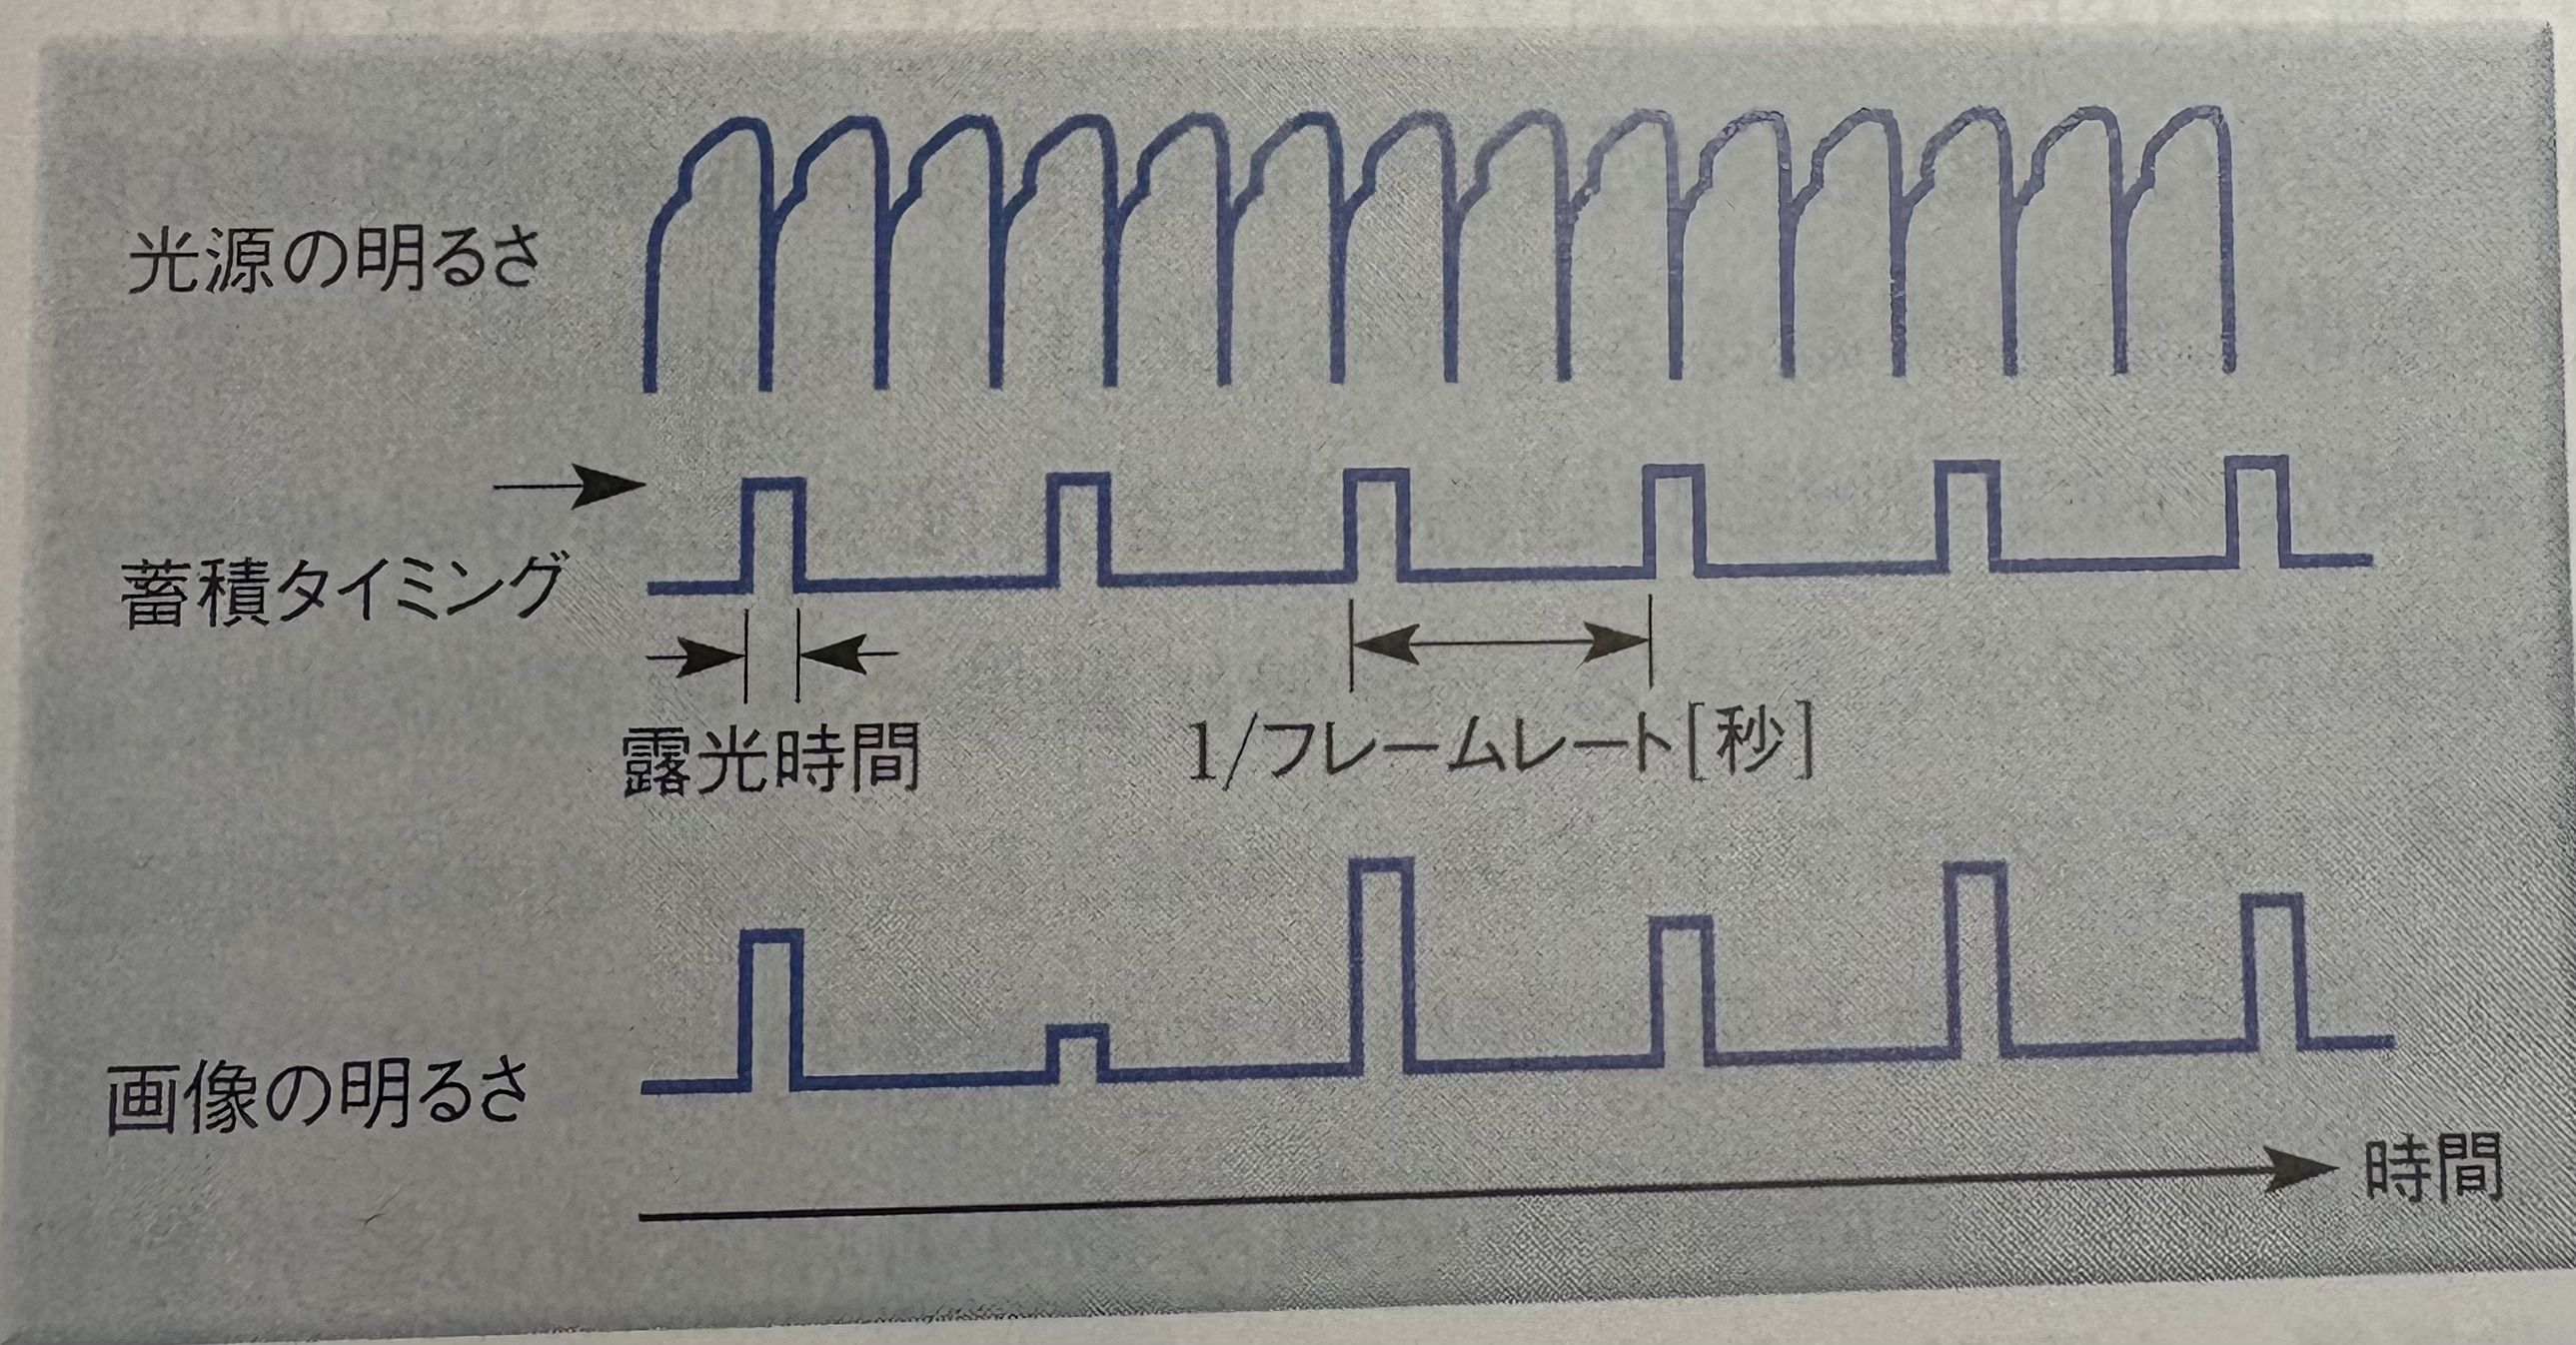
\includegraphics[width=0.5\textwidth]{figure/012.jpg}
      \caption{フリッカの発生過程}
      \label{fig:label}
  \end{figure}
\end{frame}
% \appendix

% \section{付録}



\begin{frame}[allowframebreaks]{参考文献}
  \beamertemplatetextbibitems
	\bibliographystyle{jplain}
  \nocite{*}
	\bibliography{Reference/ref1}
\end{frame}

\end{document}